\documentclass{article}

\usepackage[french]{babel}
\usepackage[T1]{fontenc}
\usepackage{moreverb}       % verbatim with tab

% https://tug.org/FontCatalogue/libertinusserif/
%\usepackage{libertinus}
%\usepackage[T1]{fontenc}
\usepackage{libertine} % Police Linux Libertine en sérif, Linux Biolinum en sans-sérif.
\usepackage[libertine]{newtxmath} % Math avec la police Libertine
%\addtokomafont{disposition}{\normalfont\sffamily} % Police des titres (ajouter \normalfont pour enlever le bold)
%\addtokomafont{paragraph}{\bfseries} % Titre des paragraphes en gras
%\addtokomafont{subsubsection}{\bfseries} % Titre des subsubsections en gras
%\usepackage[scaled=.8]{beramono} % Police monospace

\AtBeginDocument{
    \def\labelitemi{\textbullet}    % Redéfinition des puces dans les itemize
    \renewcommand{\times}{\text{×}} % Remplacer le gros «X» par un plus beau
    %\interfootnotelinepenalty=10000
}
\renewcommand\ttdefault{cmvtt}

\usepackage{wrapfig}
\usepackage{graphicx}
\usepackage{geometry}
\geometry{hmargin=2.5cm}
\usepackage{amsmath}
\usepackage{siunitx}

\usepackage{graphicx}
\usepackage{subcaption}
\usepackage{float}
\usepackage{hyperref}
\usepackage{setspace}
\usepackage{xcolor}
\usepackage{pdfpages}
\usepackage{enumitem}
\usepackage{lscape}

\usepackage{fancyhdr}       % en-têtes
\usepackage{lastpage}       % numéro de dernière page

\usepackage{booktabs}
\usepackage{dcolumn}
\newcolumntype{M}[1]{>{\centering\arraybackslash}m{#1}}


\title{Développement d'un codec audio AAC : optimisation de l'algorithme MDCT pour une architecture ARM}
\date{2020 -- 2021}
\author{Laura Binacchi}

\pagestyle{fancy}
\renewcommand\headrulewidth{1pt}
\fancyhead[L]{Laura Binacchi}
\fancyhead[C]{Développement d'un codec audio AAC}
\fancyhead[R]{2021 -- 2022}


\begin{document}
    \pagenumbering{gobble}
    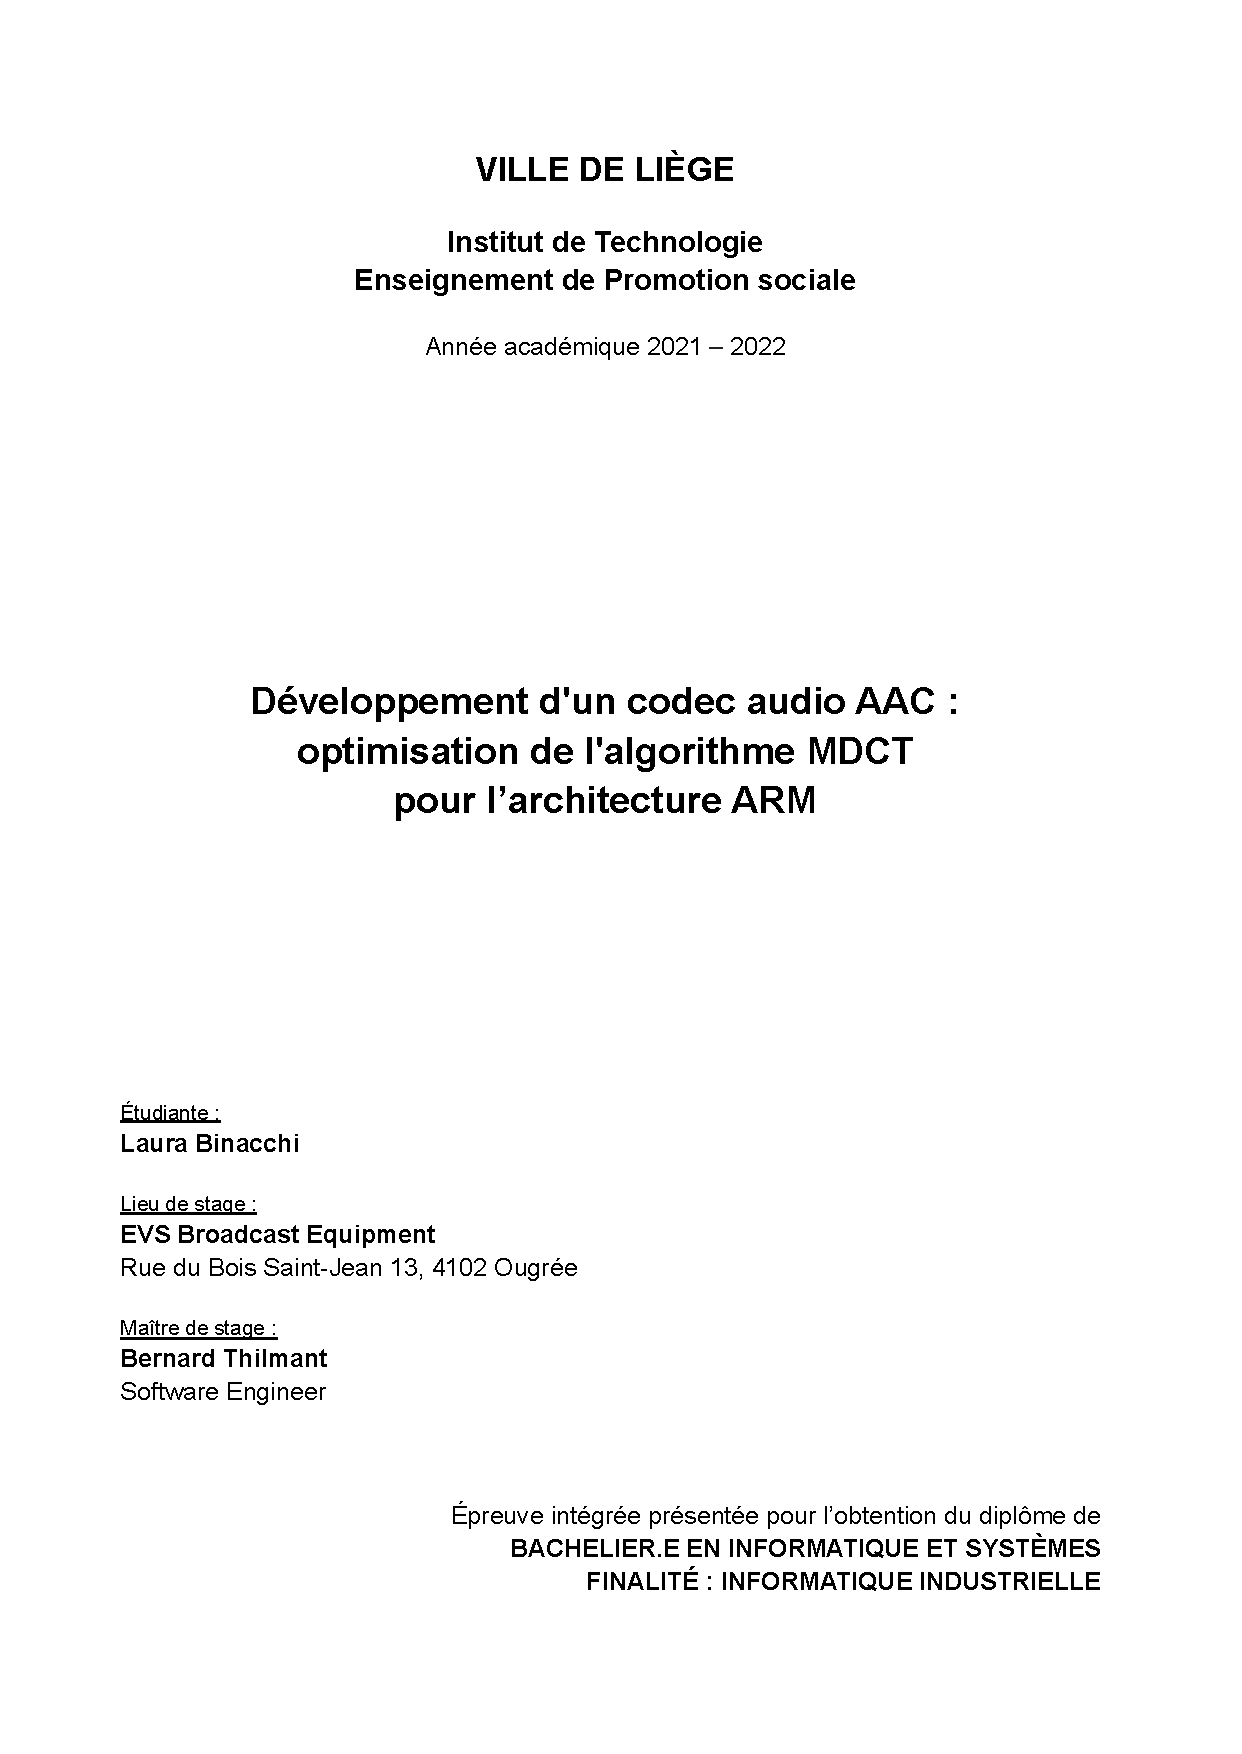
\includepdf[pages={1}]{pdg}
    \newpage
    \tableofcontents
    \newpage
    \listoffigures

    \newpage
    \section*{Remerciements}
    % TODO

    \newpage
    \pagenumbering{arabic}
    \section*{Introduction}
    \addcontentsline{toc}{section}{\protect\numberline{}Introduction}

    % Contexte du projet : serveur XT (XT VIA qui succède à ...) et passage d'une architecture Intel à une architecture ARM
    % Travail qui s'inscrit dans la continuité d'un travail théorique préalable
    % Optimisations possibles et choix de l'algorithme MDCT (mais on pourrait aussi faire la même chose pour le bloc quantization, etc.)
    % Optimisations du bloc MDCT mises en place : passage d'une arithmétique floating à fixed point et utilisation des fonctions SIMD qui offrent une meilleur capacité de calcul
    % Limite de l'optimisation : limite de temps (temps du stage) plutôt que gain de performance par rapport à ce qui est déjà en prod

    \paragraph{}
    Développement d'une solution de software embarqué sur processeur ARM pour encodage audio AAC optimisé aux applications d'EVS :
    \begin{itemize}
        \item Prise de connaissance de l'encodage AAC et de l'environnement EVS qui utilise ce type de format ;
        \item Prise de connaissance des résultats des optimisations possibles du modèle psycho-acoustique développé par EVS ;
        \item Développement du code en C ou Assembler pour l'encodage AAC sur plateforme ARM ;
        \item Test du système et documentation de son implémentation.
    \end{itemize}

    % mettre en avant le côté pratique de mon travail + dans la présentation orale

    \paragraph{}
    % sur base du cahier des charges, il a été décidé avec les personnes qui ont supervisé mon travail de me consacrer à l'optimisation du bloc MDCT

    \paragraph{}
    %Mon travail s'inscrit dans la continuité de celui de Wafaa Heddari, stagiaire qui m'a précédée au sein du département hardware-firmware d'EVS pour y travailler sur le codec AAC. Après une étude du codec AAC et des différents blocs qui le composent, son mémoire dégage des pistes d'amélioration des performances du codec AAC : like Removal of block switching, Fast MDCT, and Optimized TNS. And then test their implementation on C Code to compare the compilation speed between the original Codec and the optimized one\cite{Wafaa}.

    %L'amélioration des performances est nécessaire par la qualité grandissante des données audio et video -> de plus en plus grandes, et le besoin de maintenir plusieurs flux en tant réel dans le broadcast

    % \paragraph{}
    % Ce travail commencera par une présentation d'EVS et du département dans lequel s'est déroulé mon stage. Parmi les nombreux produits d'EVS, seul le serveur XT sera brièvement présenté puisque c'est spécifiquement pour ce dernier que le codec AAC est développé et optimisé.

    % \paragraph{}
    % Quelques notions théoriques indispensables à la compréhension du travail pratique seront ensuite développées avec une section consacrée au son et sa numérisation et une autre consacrée aux codecs MPEG, à leur fonctionnement et en particulier au fonctionnement du bloc MDCT de l'encodeur AAC.

    % But : garder la max de performance en perdant le moins en qualité


    %\paragraph{}
    %Si les sections de présentation des différentes itérations de la MDCT ont déjà permis de mettre en avant certains résultats en terme de performance ou de précision, c'est la section suivante qui présentera la protocole de valitation ainsi que les résultats obtenus pour la version finale de l'algorithme MDCT en \emph{integer}.

    % présenter les annexes et dire laquelle est la plus importante l'annexe x ets particulièrement à souligner car + importante

    \newpage
    \section{EVS Broadcast Equipment}
    \subsection{Présentation d'EVS et du département R\&D}
    \paragraph{}
    Mon stage s'est déroulé au sein de la société EVS Broadcast Equipment dont la figure \ref{fig:logo} représente le logo. EVS est une entreprise d'origine liégeoise devenue internationale. Fondée en 1994 par Pierre L'Hoest, Laurent Minguet et Michel Counson, EVS compte aujourd'hui plus de 600 employés dans plus de 20 bureaux à travers le monde mais son siège principal se situe toujours à Liège\cite{EVS:website}.

    \begin{figure}[H]
        \centering
        
\includegraphics[width=.5\linewidth]{./images/EVS-logo.png}
        \caption{Logo de la société EVS Broadcast Equipment}
        \label{fig:logo}
    \end{figure}

    \paragraph{}
    EVS est devenu leader dans le monde du broadcast avec ses serveurs permettant l'accès et la diffusion instantanée des données audiovisuelles enregistrées sur ses serveurs. L'entreprise est également célèbre pour ses ralentis instantanés. Ces technologies sont utilisées pour la production live des plus importants événements sportifs dans le monde : le matériel EVS est notamment utilisé pour la retransmission des Jeux Olympiques depuis 1998.

    \paragraph{}
    Plus de 50\% des employés d'EVS travaillent en recherche et développement afin de répondre au marché du broadcast en constante évolution. Outre ses solutions techniques innovantes, EVS se différencie de ses concurrents par la proximité entretenue avec les clients en leur proposant des solutions à l'écoute de leurs besoins et en leur offrant un service de support de qualité.

    \paragraph{}
    C'est en R\&D, dans l'équipe Hardware-Firmware, que s'est déroulé mon stage. Sous la direction de Justin Mannesberg, cette équipe se compose d'une vingtaine d'employés spécialisés en développement embarqué et en développement FPGA. La situation particulière dans laquelle s'est déroulé mon stage, en pleine pandémie de Covid et alors que tous les employés étaient confinés, ne m'a pas permis d'interagir avec beaucoup de membres de l'équipe et ni de pouvoir observer leur travail. Bernard Thilmant (Software Engineer dans l'équipe Hardware-Firmware) a cependant réussi à m'apporter le soutien nécessaire à la bonne réalisation de mon stage : il m'a permis de m'initier au C++, m'a aidée à ne pas me perdre dans les concepts parfois complexes de l'encodage audio et m'a aidée à apporter la rigueur scientifique nécessaire à la réalisation de mon travail. J'ai également pu bénéficier de l'expertise technique de Frédéric Lefranc (Principal Embedded System Architect dans l'équipe Hardware-Firmware) ainsi que du suivi de Justin Mannesberg (Manager de l'équipe Hardware-Firmware).

    \subsection{Le serveur XT}
    \paragraph{}
    EVS développe et commercialise de nombreux produits allant des serveurs de production aux interfaces permettant d'exploiter des données audiovisuelles ou de monitorer des systèmes de production\cite{EVS:products}. Le serveur de production live XT est un des produits emblématiques d'EVS. Il permet de stocker de grandes quantités de données audiovisuelles et d'y accéder en temps réel afin de répondre aux besoins de la production en live. Par exemple, la remote LSM (\emph{Live Slow Motion} permet d'accéder aux contenus des serveurs XT afin de créer les ralentis pour lesquels EVS est célèbre dans le monde.

    \begin{figure}[H]
        \centering
        \begin{subfigure}[b]{0.4\linewidth}
            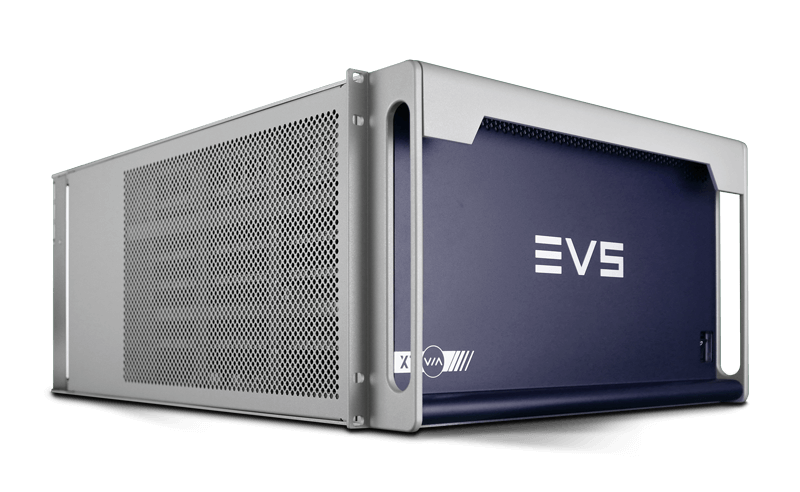
\includegraphics[width=\linewidth]{./images/XT-VIA.png}
        \end{subfigure}
        \begin{subfigure}[b]{0.4\linewidth}
            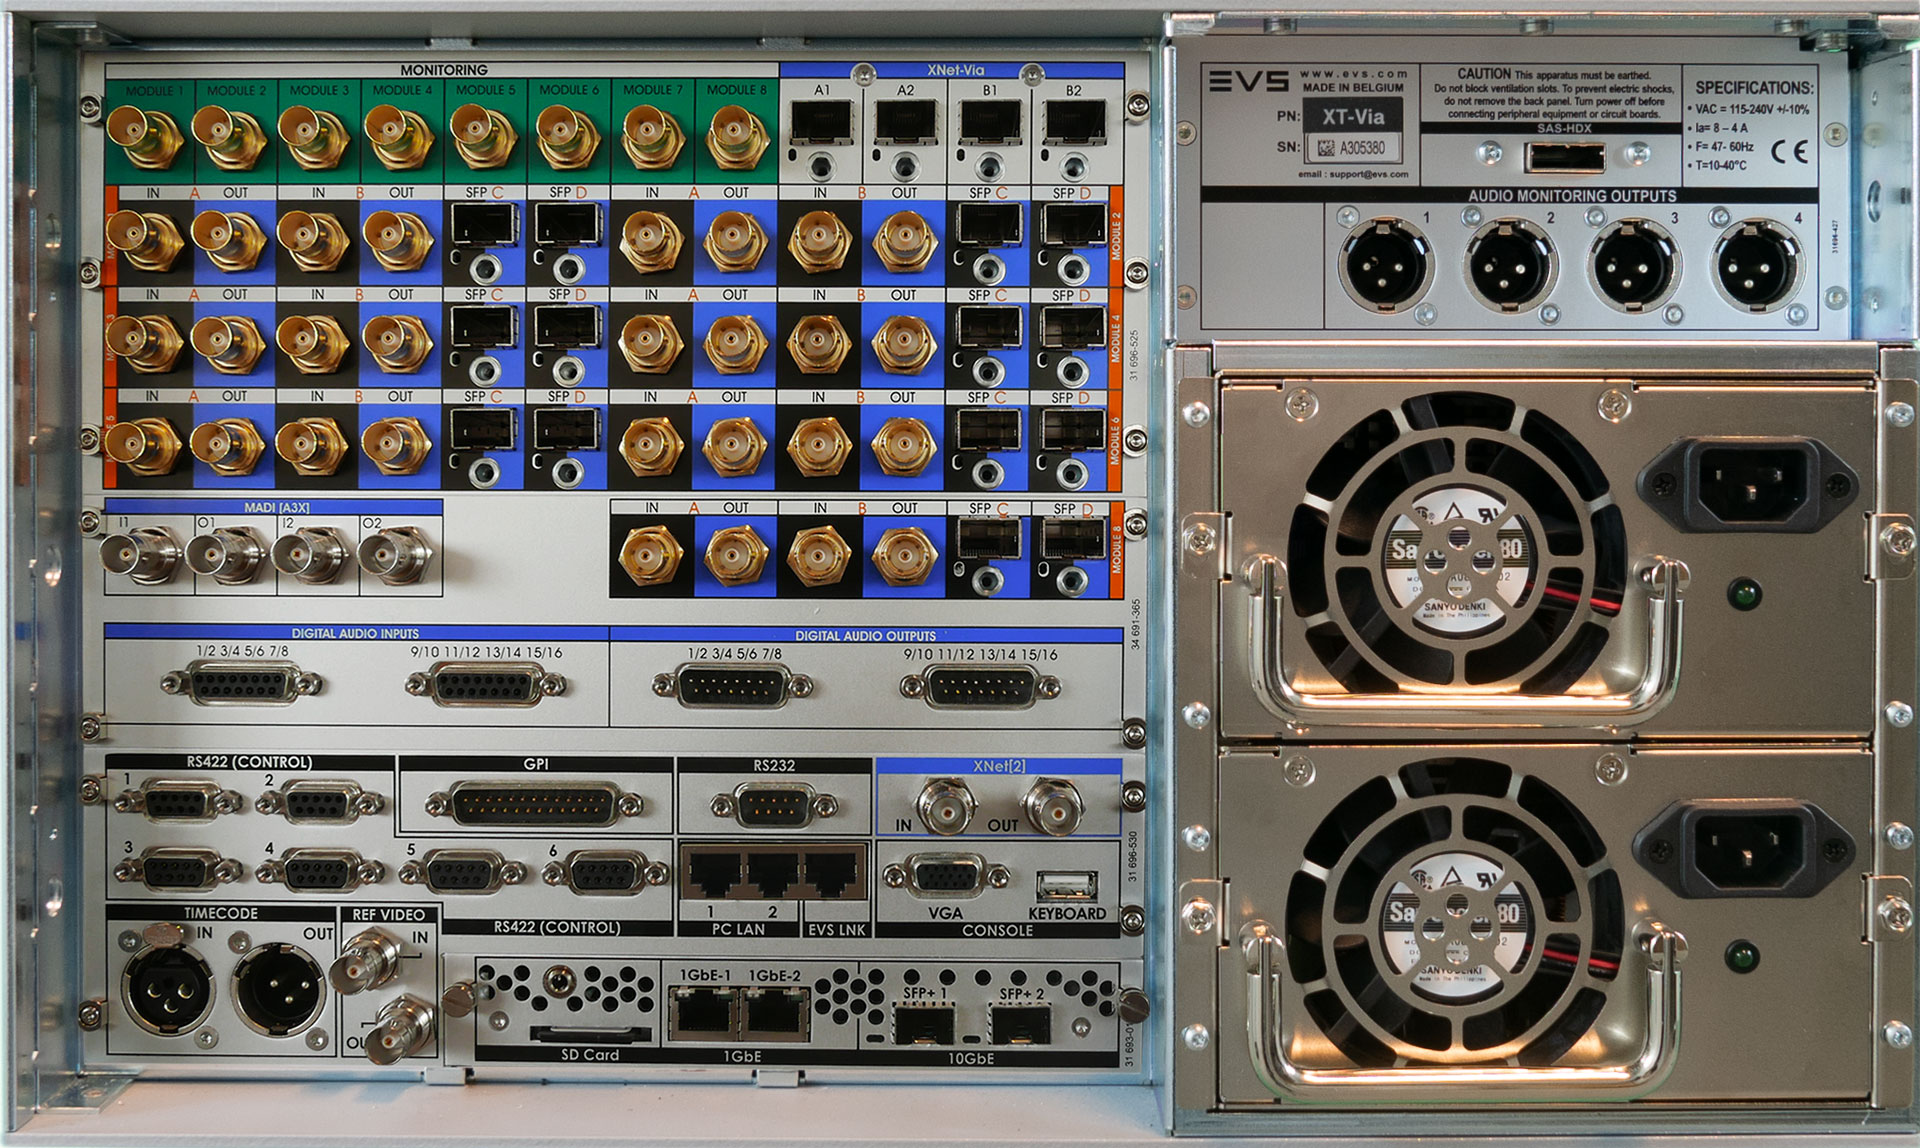
\includegraphics[width=\linewidth]{./images/XT-VIA-ar.jpg}
        \end{subfigure}
        \caption{Vues avant et arrière (en configuration IP) de l'XT-VIA}
        \label{fig:xt-via}
    \end{figure} 

    \paragraph{}
    Le serveur XT a connu plusieurs versions : XT, XT2, XT2+, XT3 et enfin l'XT-VIA. L'XT-VIA (cf figure \ref{fig:xt-via}), la plus récente version du serveur XT, en quelques informations clés\cite{EVS:products} :
    \begin{itemize}
        \item offre un espace de stockage de 18 à 54 TB, soit plus de 130h d'enregistrement en UHD-4K;
        \item dispose de 2 à plus de 16 canaux selon le format choisi : 2 canaux en UHD-8K (4320p), 6 canaux en UHD-4K (2160p) et plus de 16 canaux en FHD and HD (720p, 1080i, 1080p);
        \item permet une configuration hybride de ses entrées et sorties en IP (10G Ethernet SFP+, 100G en option, ST2022-6, ST2022-7, ST2022-8, ST2110, NMOS IS-04, IS-05, EMBER+, PTP) ou SDI (1.5G-SDI, 3G-SDI et 12G-SDI);
        \item supporte de nombreux formats d'encodage vidéo : UHD-4K (XAVC-Intra et DNxHR), HD/FHD (XAVC-I, AVC-I, DNxHD et ProRes), PROXY (MJPEG et H264);
        \item peut enregistrer 192 canaux audio non compressés et supporte les standards AES et MADI;
        \item offre de nombreuses possibilités de connexion avec du matériel EVS ou non.
    \end{itemize}

    \paragraph{}
    C'est pour la dernière génération du serveur XT, l'XT-VIA, que le codec AAC est développé. La compression avec perte de données de ce codec permet d'optimiser l'espace occupé par les données audio sans en altérer la qualité perçue. Outre la qualité audio, les performances de l'encodage sont importantes à prendre en compte pour permettre l'enregistrement de plusieurs canaux en parallèle tout en conservant un traitement de l'information qui tienne le temps réel. L'optimisation des performances doit tenir compte de l'architecture de l'XT-VIA : l'architecture ARM Neon remplace l'architecture Intel x86 de ses prédécesseurs avec des différences importantes dans les fonctions intrinsèques.


    \newpage
    \section{L'encodage audionumérique : généralités}
    \subsection{Le son}
    % onde acoustique -> 

    % - son audible = vibration entre 20 et 20kHz

    % le signal, analogique (continu) ou discret, peut avoir une représentation :
    % - temporelle
    % - fréquentielle
    % exemple de signaux périodiques (sinus, carré, etc) -> pp 6-7 + truc interactif

    % - spectre d'amplitude (utile) et spectre de phase (pas utile)

    % - toute fonction p(x, t) peut être exprimée par une somme de fonctions (co-)sinusoidales : formule pour les fonctions périodiques + transformée de Fourier pour les fonctions n'est pas périodique dans le temps

    \subsection{La numérisation d'un signal}
    \label{audionumerique}
    % transformation de fourier :
    % https://www.claudegabriel.be/Math%C3%A9matiques%20appliqu%C3%A9es,%20chapitre%204.pdf -> p12 sur N pair / impair
    % à la base -> signaux périodique (faire bref)
    % -> ce qui nous intéresse : transformation pour signal non périodique discret -> DCT


    \newpage
    \section{Les codecs audio}
    \subsection{Définition d'un codec}
    \paragraph{}
    Un codec est un procédé logiciel composé d'un encodeur (\emph{\textbf{co}der}) et d'un décodeur (\emph{\textbf{dec}oder})\cite{wiki:codec}. Un codec audio permet donc, d'une part, de coder un signal audio dans un flux de données numériques et, d'autre part, de décoder ces données afin de restituer le signal audio.

    \paragraph{}
    Les codecs sont dits avec perte (\emph{lossy}) ou sans perte (\emph{lossless}). Le PCM est par exemple un codec sans perte puisqu'il encode la totalité des informations sonores dans la bande de fréquences humainement audible. Ce type de codec permet de conserver la qualité de l'audio mais nécessite en contrepartie un espace de stockage conséquent, même avec une compression des données.

    \paragraph{}
    Afin de réduire l'espace de stockage nécessaire, les codecs avec perte permettent de supprimer une partie des données audio. C'est le cas des codecs définis par les normes MPEG dont fait partie le codec AAC.

    \subsection{Les codecs MPEG}
    \paragraph{}
    MPEG (\emph{Moving Picture Experts Group}) désigne une alliance de différents groupes de travail définissant des normes d'encodage, de compression et décompression et de transmission de média audio, vidéo et graphiques\cite{wiki:MPEG}. Le groupe est actif depuis 1988 et a produit depuis de nombreuses normes.

    \paragraph{}
    Les codecs audio qui implémentent les normes MPEG ont pour point commun d'être des codecs avec perte de données basés sur un modèle psychoacoustique. Le premier est le MP3, défini par la norme MPEG-1 Layer-3 ISO/IEC 11172-3:1993. Le codec AAC est conçu en 1997 pour remplacer le MP3. Il est défini par les normes MPEG-2 partie 7 ISO/IEC 13818-7:2006\cite{ISO13818-7} et MPEG-4 partie 3 ISO/IEC 14496-3:2019\cite{ISO14496-3}.

    \paragraph{}
    Les normes MPEG définissent les grandes lignes de l'encodage et du décodage et le format du conteneur mais pas l'implémentation du codec qui peut de ce fait être plus ou moins performant. Les codecs MPEG sont typiquement composés des blocs suivants\cite{1999-Brandenburg} :
    \begin{figure}[H]
        \centering
        \begin{subfigure}[b]{.6\linewidth}
            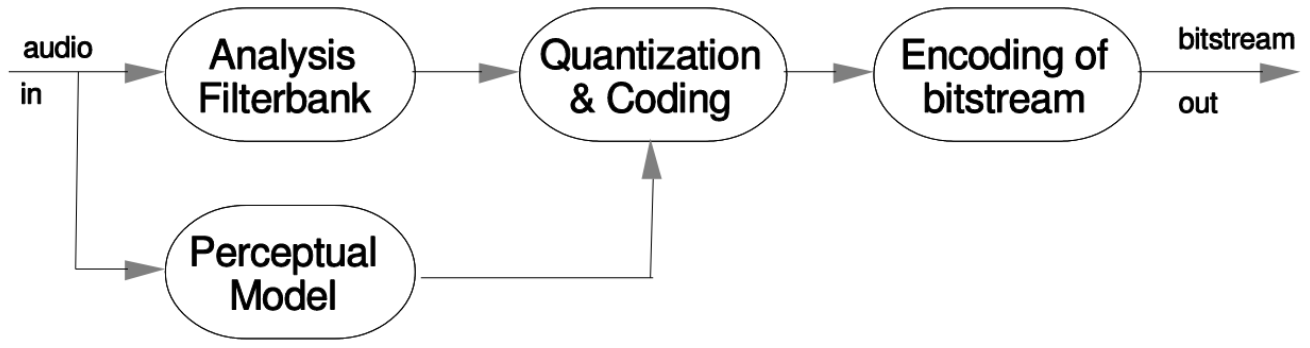
\includegraphics[width=\linewidth]{./images/1999-Brandenburg-simple-AAC-encoder.png}
            \caption{Schéma fonctionnel de l'encodeur}
        \end{subfigure}
        \begin{subfigure}[b]{.6\linewidth}
            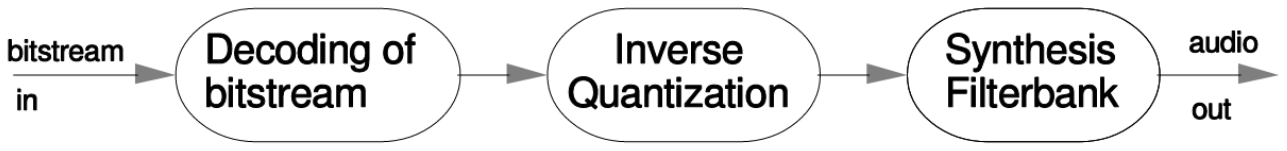
\includegraphics[width=\linewidth]{./images/1999-Brandenburg-simple-AAC-decoder.png}
            \caption{Schéma fonctionnel du décodeur}
        \end{subfigure}
        \caption{Vue simplifiée d'un codec MPEG basé sur un modèle psychoacoustique}
    \end{figure}
    \paragraph{}
    L'encodeur est composé des blocs suivants :
    \begin{description}
        \item[filter bank] la banque de filtres décompose le signal temporel d'entrée en différentes composantes fréquentielles
        \item[perceptual model] le modèle psychoacoustique utilise le signal temporel et/ou sa décomposition fréquentielle pour éliminer les données audio dont l'absence ne nuira pas à la qualité perçue à l'écoute ()
        \item[quantization and coding] la quantification attribue une valeur numérique aux données du spectre de fréquences : elles sont typiquement codées avec une méthode entropique qui peut être optimisée avec le modèle psychoacoustique
        \item[encoding of bitstream] les données sont formatées en un flux contenant typiquement le spectre de fréquences codé et des informations supplémentaires permettant l'encodage
    \end{description}
    
    \paragraph{}
    Le décodeur a un fonctionnement inverse : le flux de données est décodé (\textbf{decoding of bitstream}), les composantes fréquentielles du signal sont retrouvées par l'opération inverse à la quantification (\textbf{inverse quantization}) et ces sous-bandes fréquentielles sont finalement rassemblées pour reconstituer le signal temporel (\textbf{synthesis filter bank}).

    \paragraph{}
    Le fonctionnement du décodeur ne sera pas plus développé dans ce travail car le bloc MDCT fait partie de la banque de filtres de l'encodeur. Le fonctionnement spécifique de l'encodeur AAC sera par contre détaillé dans la section \ref{sec:AAC}.


    \subsection{Les modèles psychoacoustiques}
    \paragraph{}
    Le section précédente a défini les codecs MPEG comme étant basés sur un modèle psychoacoustique. La psychoacoustique est une branche de la psychophysique qui étudie la manière dont l'oreille humaine perçoit le son\cite{wiki:psychoacoustic}. Cette discipline permet d'améliorer la compression d'un signal audio en éliminant les sons qui sont captés par un microphone mais qui ne peuvent pas être perçus par l'oreille humaine et les avancées dans cette discipline permettent de développer des encodeurs audio de plus en plus performants. Les codecs basés sur un modèle psychoacoustique sont toujours des codecs avec perte puisqu'une partie des informations auditives sera définitivement perdue, ce qui ne nuit pour autant pas à la qualité perçue du son.

    \paragraph{}
    L'encodage audionumérique tient déjà compte des seuils de fréquences humainement audibles pour limiter les données audio enregistrées : nous l'avons vu dans la section \ref{audionumerique}, aucun son n'est perçu en-deça de \SI{20}{\hertz} ou au-delà de \SI{20}{\kilo\hertz}. La psychoacoustique permet de mieux dessiner la limite entre ce qui est humainement audible ou non afin d'éliminer un maximum des informations non pertinentes et ainsi augmenter le facteur de compression des données : le facteur de compression des codecs MPEG est environ 15 fois supérieur à celui du CD\cite{2019-Herre-Dick}.

    \paragraph{}
    Les effets de masque sont au centre des différents modèles psychoacoustiques utilisés pour la compression audio. L'enjeu afin d'obtenir le meilleur taux de compression est de calculer le plus finement possible les seuils de masquage, i.e. la limite entre les informations pertinentes et celles qui peuvent être éliminées. Les effets de masques dans le domaine fréquentiel (\emph{spectral masking effects}) sont parmi les plus utilisés mais il en existe d'autres, e.g. dans le domaine temporel. La figure suivante représente différents effets de masque du domaine fréquentiel :
    \begin{figure}[H]
        \centering
        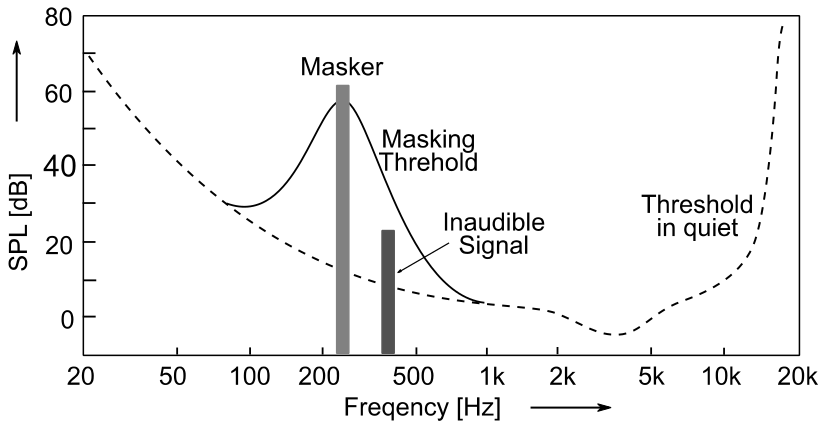
\includegraphics[width=.6\linewidth]{./images/2019-Herre-Dick-masking-effect.png}
        \caption{Effets de masque dans le domaine fréquentiel}
    \end{figure}

    % \paragraph{}
    % Les lignes représentent le seuil 
    % \begin{description}
    %     \item[Threshold in quiet] la ligne en pointillé représente le seuil d'audibilité dans le calme, indépendamment de tout autre élément qui pourrait interférer
    %     \item[Masking threshold] 
    % \end{description}


    % SPL) A frequency dependent threshold of in hearing in quiet describes the minimum sound pressure level of a sound to be perceivable isolation and under extremely quite conditions. (SPL) of a sound be perceivable in isolation and curve under extremely conditions. • In the presence of to a masker, the threshold in quiet changes into quite a masking threshold, which bell-shaped increase the in frequencies the vicinity of the masker, depending on its • shows In the a presence of a masker, threshold in in quiet curve changes into a masking threshold, frequency, level, and signal increase type. Any sound beneath threshold is masked by the louder which shows a bell-shaped in frequencies in the this vicinity of the masker, depending on its signal, and level, thus and inaudible the Any average perceptual coding, the louder coding signal, error frequency, signal for type. sound listener. beneath In this threshold audio is masked by the (i.e., the introduced quantization noise) corresponds to the probe signal in this experimental and thus inaudible for the average listener. In perceptual audio coding, the coding error (i.e., scenario. the introduced quantization noise) corresponds to the probe signal in this experimental scenario. • Masking effects are are strongest strongest signals are within the critical bandwidth of the masker. • Masking effects for for signals that that are within the critical bandwidth of the masker. Within Within the critical bandwidth, the masking threshold remains constant. Furthermore, the the critical bandwidth, the masking threshold remains constant. Furthermore, the masking effects masking spread to frequencies the (so-called critical bandwidth (so-called The inter-band spread to effects frequencies beyond the critical beyond bandwidth inter-band masking). upper masking). The upper slope of the masking threshold depends on multiple factors, such as absolute slope of the masking threshold depends on multiple factors, such as absolute frequency and sound frequency and of sound pressure whereas level of the the lower masker, whereas lower slope dependency. hardly shows a level pressure level the masker, slope hardly the shows a level dependency. • Depending on the type of masker, i.e., tone or (narrow-band) noise, the strength of the masking • Depending the type of masker, i.e., can tone or (narrow-band) the strength of the masking effect varies. on While noise-like maskers mask tone-like signals noise, very well (up to a masker-to-probe effect varies. maskers can mask tone-like signals very well (up to a masker-to- level ratio of While about noise-like 6 dB), tone-like maskers can mask noise only to a much weaker extent [29] probe level ratio of about 6 dB), tone-like maskers can mask noise only to a much weaker extent (about 20 dB). [29] (about 20 dB).      \paragraph{}     Le calcul des   


    
    
    
    % Le calcul du seuil de masquage tient compte\cite{2019-Herre-Dick} :
    % \begin{itemize}
    %     \item des effets de masquage monophonique de la perception non-linéaire des fréquences, plus fine pour les basses fréquences;
    %     \item des effets de masque dans le temps;
    %     \item de l'effet de masque dans une bande de fréquence ou entre bandes de fréquences;
    %     \item l'impact de la tonalité sur le masquage
    %     \item masking over time
    % \end{itemize}


    \newpage
    \section{Le codec AAC}
    \label{sec:AAC}
    \subsection{Fonctionnement de l'encodeur AAC}
    % présentation des différents blocs
    % \cite{wiki:AAC}

    %In this thesis, we are going to study the different blocks of an AAC encoder based on the standard ISO/IEC 13818-7 such as the psychoacoustic model, Gain control, Transform block, Spectral processing, Quantization and Entropy coding. \cite{Wafaa}

    % Les codecs définis par les normes MPEG sont basés sur le modèle psychoacoustiquev
    % Les performances des codecs audio définis par les normes MPEG sont rendues possibles par les recherches en psychoacoustique.


    %AAC supports inclusion of 48 full-bandwidth (up to 96 kHz) audio channels in one stream plus 16 low frequency effects (LFE, limited to 120 Hz) channels, up to 16 "coupling" or dialog channels, and up to 16 data streams. The quality for stereo is satisfactory to modest requirements at 96 kbit/s in joint stereo mode; however, hi-fi transparency demands data rates of at least 128 kbit/s (VBR). Tests[which?] of MPEG-4 audio have shown that AAC meets the requirements referred to as "transparent" for the ITU at 128 kbit/s for stereo, and 320 kbit/s for 5.1 audio.[citation needed] 
    % AAC uses only a modified discrete cosine transform (MDCT) algorithm, giving it higher compression efficiency than MP3, which uses a hybrid coding algorithm that is part MDCT and part FFT.[4]


    % \paragraph{}
    % Le codec AAC (Advanced Audio coding) est définit  , défini par la norme . Les recherches en psychoacoustique ont permis de développer un algorithme d'encodage plus performant pour l'AAC que pour le MP3 : il permet d'encoder moins de données audio tout en gardant la même qualité perçue au décodage\cite{1999-Brandenburg}.



    \subsection{Le bloc MDCT}
    % \begin{itemize}
    %     \item particularités par rapport à la FFT
    %     \item basée sur la DCT-IV
    %     \item niveaux de complexité (O...)
    % \end{itemize}

    % faire un scema fonctionnel des 3 blocs de l'implementation de MDCT choisie : pre-processig - FFT - post-processing


    \newpage
    \section{Environnement de développement}
    % \paragraph{}
    % Plateformes : passage de Intel à ARM nécessaire à cause de la lib Ne10 et impossibilité de maintenir une version de référence Intel

    % \paragraph{}
    % Développement remote sur RPI + photo raspberry

    % \paragraph{}
    % CentOS7 parce que utilisé sur tout le matériel linux EVS

    % \paragraph{}
    % Projet en C++ mais qui ressemble fort à du C car implémentation d'un codec -> améliorations possibles : juste du C ?

    % \paragraph{}
    % Le build du projet se fait grâce à un fichier CMake à la racine du projet. Ce fichier présenté dans l'annexe \ref{an:cmake_super} permet d'appeler les CMake du projet \emph{audio\_encoding} (projet contenant les MDCT et ses tests) et de la librairie \emph{Ne10}. Les commandes du CMake générant les exécutables de tests seront fournies en annexe à la suite du code source de ces tests.



    \newpage
    \section{Algorithmes MDCT de référence}

    \paragraph{}
    La première étape de ce travail consiste à développer des algorithmes de référence afin de valider les différentes MDCT implémentées par la suite. Ces algorithmes de référence sont développés en algorithmique flottante sur base de la formule mathématique de la MDCT. Ils permettent de générer des spectres de fréquences en \emph{float} ou en \emph{integer} afin de valider les données de sortie des MDCT optimisées.


    \subsection{Description mathématique}
    \label{sec:desc-math}

    \paragraph{}
    La transformation effectuée par la MDCT est donnée par l'équation suivante\cite{wiki:MDCT} :
    $$X_k = \sum_{n=0}^{2N-1} x_n \cos \left[ \frac{\pi}{N} \left( N + \frac{1}{2} + \frac{N}{2} \right) \left( k + \frac{1}{2} \right) \right]$$
    \begin{description}
        \item[$X_k$] avec $k \in [0, N[$ pour une fenêtre d'entrée de 2N échantillons
        \item[$x_n$] avec $n \in [0, 2N[$ : la fenêtre d'entrée
        \item[$F: R^{2N} \rightarrow R^N$] la MDCT est une fonction linéaire qui pour 2N nombres réels en entrée produit N nombres réels en sortie
    \end{description}\label{test}

    \paragraph{}
    À cette équation s'ajoute le facteur d'échelle $\frac{2}{\sqrt{2N}}$.

    \paragraph{}
    La MDCT a été implémentée avec une fenêtre d'entrée de $2N = 1024$ échantillons. Le bloc de sortie, i.e. le spectre de fréquences de la fenêtre d'entrée, aura donc une taille de 512. Ces valeurs, utilisées à de très nombreux endroits du code, sont rassemblées dans le header \texttt{mdct\_constants.h} présenté dans l'\textbf{annexe B}. Ce fichier contient également d'autres valeurs précalculées sur base de la taille de la fenêtre d'entrée.

    \paragraph{}
    La section suivante présente deux implémentations simples de cette formule. Ces implémentations ne pourraient pas être utilisées sans avoir été optimisées car elles seraient beaucoup trop lentes pour un codec qui doit tenir le temps réel sur plusieurs canaux. La complexité de l'implémentation de cette formule est de $O(N^2)$ opérations (où N est la taille de la fenêtre d'entrée). Cette complexité peut être ramenée à $O(N \log N)$ opérations par une factorisation récursive. La complexité peut également être diminuée en se basant sur une autre transformation, e.g. une DFT (\emph{Discrete Fourier Transorm}) ou une autre DCT (\emph{Discrete Cosine Transform}) : la complexité sera alors de $O(N)$ opérations de \emph{pre-} et \emph{post-processing} en plus de la complexité de la DFT ou de la DCT choisie\cite{wiki:MDCT}. C'est cette dernière option qui a été retenue pour ce travail.

    \subsection{Implémentations des MDCT de référence en \emph{floating point} et \emph{fixed point}}

    \paragraph{}
    La formule mathématique de la MDCT a été implémentée très simplement en algorithmique flottante avec la possibilité d'obtenir le spectre de fréquences codé en \emph{float}, \emph{double} ou \emph{int32}. L'objectif de ces implémentations est de pouvoir valider les spectres de fréquences calculés par les implémentations optimisées de la MDCT. Les MDCT de référence serviront également à mesurer la précision des MDCT optimisées.

    \paragraph{}
    La première implémentation de l'équation de la MDCT est présentée dans l'\textbf{annexe C.1}. La fonction développée permet de faire ses calculs et d'obtenir un résultat aussi bien en \emph{float} (32 bits) qu'en \emph{double} (64 bits) grâce à l'utilisation d'un \emph{template}. Le signal temporel a la même précision (\emph{float} ou \emph{double}) que le spectre généré.

    \paragraph{}
    La seconde fonction de référence est présentée dans l'\textbf{annexe C.2}. Elle permettra de vérifier les résultats des implémentations optimisées en \emph{fixed point}. Tous les calculs ne sont pas fait en algorithmique entière : la fonction fait les mêmes calculs que la fonction de référence en algorithmique flottante (uniquement en \emph{double} cette fois pour garder le plus de précision possible) et transtype le résultat final dans un \emph{integer} de 32 bits qui correspond à une notation Qx.15 signée.


    \subsection{Validation}
    \paragraph{}
    Les MDCT de référence sont validées en générant le spectre de fréquences d'un signal connu pour pouvoir observer que celui-ci corresponde bien à ce qui est attendu. Tout au long de ce travail, les MDCT ont été validées avec divers signaux en entrée : des signaux à une ou plusieurs fréquences connues ou des données aléatoires. La section \ref{sec:validation} consacrée au protocole de validation donne plus de détails sur la génération des spectres de fréquences produits par les MDCT et leur interprétation. 

    \paragraph{}
    Afin de faciliter la lecture des résultats et les comparaisons, ce travail présentera principalement des tests effectués avec en entrée un signal à \SI{440}{\hertz}. L'\textbf{annexe D} présente les codes permettant de générer des signaux sinusoïdaux. Les signaux sinusoïdaux sont produits en \emph{floating point} (\textbf{annexe D.1}) ou en \emph{fixed point} (\textbf{annexe D.2}). Le signal est paramétrable :
    \begin{itemize}
        \item en taille ou nombre d'échantillons : la fenêtre d'entrée de la MDCT sera toujours de 1024 échantillons;
        \item en amplitude : paramètre utilisé pour limiter le signal un un certain \emph{range} de valeurs;
        \item en fréquence : la fréquence des exemples de résultats donnés dans ce travail sera le plus souvent de \SI{440}{\hertz} mais les MDCT ont été testées avec de nombreux autres signaux;
        \item en déphasage : ce paramètre n'a pas été utilisé;
        \item et en fréquence d'échantillonnage toujours à \SI{48}{\kilo\hertz}.
    \end{itemize}

    \paragraph{}
    La \emph{headroom} est l'espace réservé aux valeurs limites du signal : le signal réel est clippé et ne couvre pas l'ensemble des valeurs possibles. Dans ce travail, la \emph{range} du signal est toujours comprise entre $-0.9$ et $0.9$, que le signal soit codé en \emph{floating point} ou en \emph{fixed point}. Ce fait est moins important pour les algorithmes travaillant en \emph{floating point} mais il sera essentiel pour la mise à échelle des données en représentation \emph{fixed point} (section \ref{sec:fixed_point}).

    \paragraph{}
    Les signaux codés en \emph{float} ou en \emph{double} serviront à valider les implémenations intermédiaires de la MDCT. L'objectif reste cependant de développer une MDCT capable de traiter des données entières sans transtypage. Le signal en \emph{integer} servira à valider les dernières itérations de la MDCT. Ce signal est codé en 16 bits (représentation Q15 signée) afin de correspondre aux données réelles qui seront reçues par l'algorithme.

    \paragraph{}
    La figure \ref{fig:signal_f32_f64} offre une représentation graphique des signaux sinusoïdaux en \emph{floating point} utilisés pour tester les MDCT en \emph{floating point} :
    \begin{itemize}
        \item les deux signaux sont équivalents : le signal généré en \emph{float} (en pointillés) se superpose parfaitement au signal généré en \emph{double};
        \item la période du signal est de \SI{2.3}{\milli\second} correspondant à la fréquence de \SI{440}{\hertz} attendue;
        \item les valeurs du signal sont comprises entre $-0.9$ et $0.9$ pour respecter une \emph{headroom}.
    \end{itemize}

    \begin{figure}[H]
        \centering
        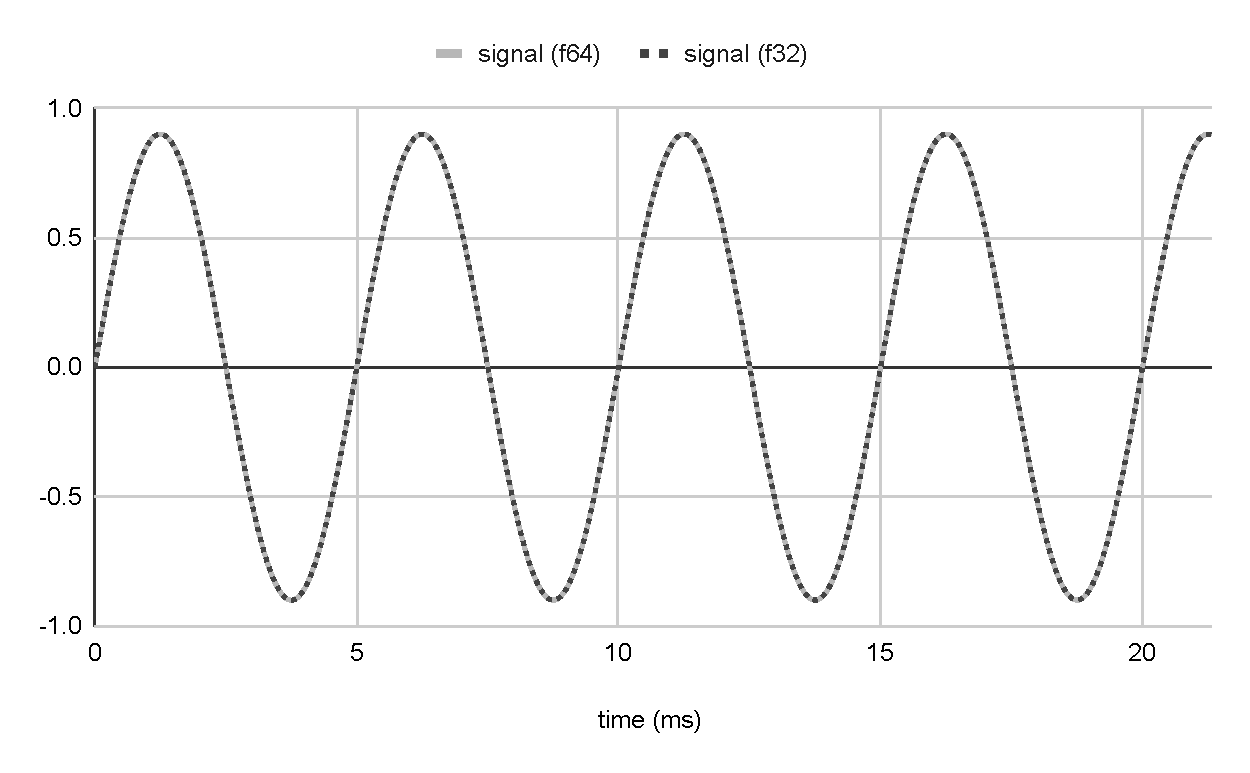
\includegraphics[width=.8\linewidth]{./images/signal_f32_f64.pdf}
        \caption{Signal sinusoïdal à \SI{440}{\hertz} codé en \emph{floating point} (\emph{float} et \emph{double})}
        \label{fig:signal_f32_f64}
    \end{figure}

    \begin{figure}[H]
        \centering
        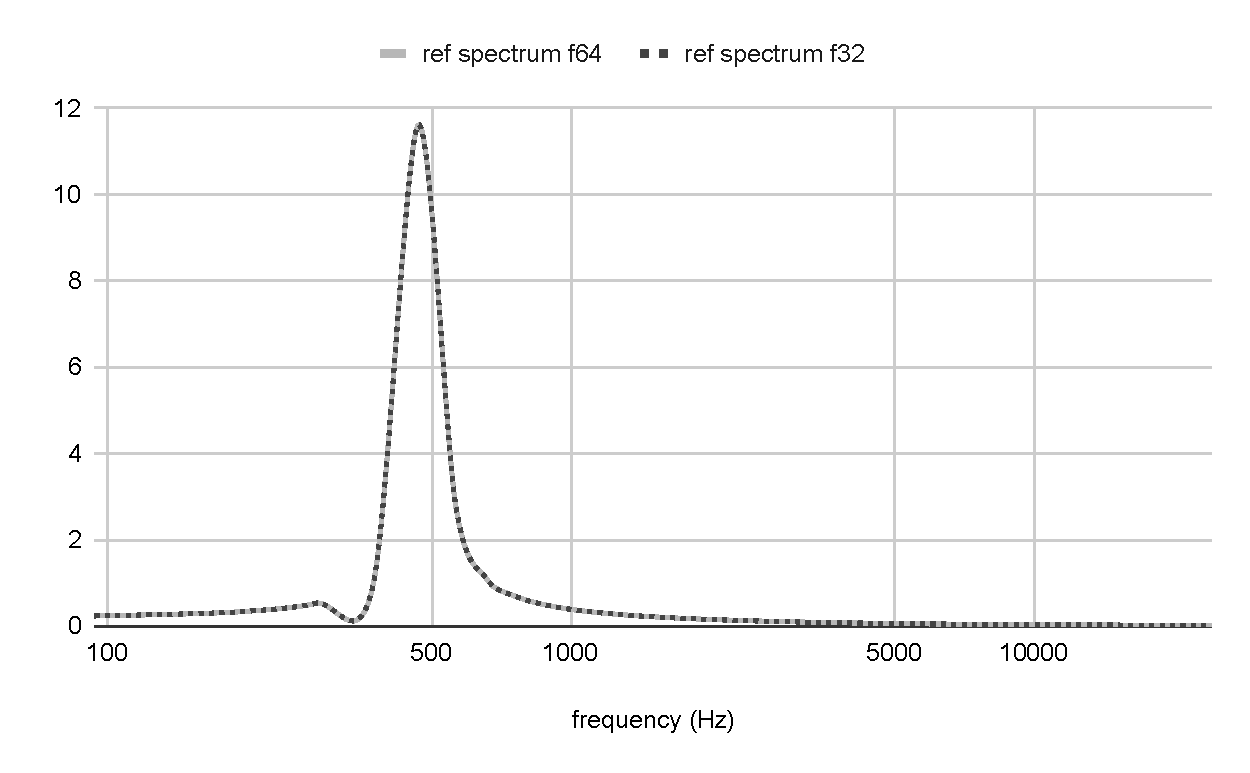
\includegraphics[width=.8\linewidth]{./images/validation_ref_float.pdf}
        \caption{Spectres de fréquences générés par les MDCT de référence en \emph{floating point}}
        \label{fig:validation_ref_mdct_float}
    \end{figure}

    \paragraph{}
    Les MDCT de référence en \emph{floating point} prenant en entrée ces signaux sinusoïdaux à \SI{440}{\hertz} génèrent les spectres de fréquences présentés à la figure \ref{fig:validation_ref_mdct_float} :
    \begin{itemize}
        \item les deux MDCT génèrent le même spectre : le spectre généré par l'agorithme en \emph{float} (en pointillés) se superpose parfaitement à celui généré en \emph{double};
        \item la représentation graphique des spectres de fréquences met bien en évidence une composante fréquentielle principale aux alentours de \SI{440}{\hertz};
    \end{itemize}

    \paragraph{}
    Le résultat obtenu est déjà satisfaisant puique la fréquence mise en évidence par le spectre est bien celle du signal d'entrée. Cependant, l'impléméntation d'une fonction de fenêtre appliquée au signal d'entrée permettrait d'améliorer encore le spectre de fréquences généré par la MDCT. La section \ref{sec:ameliorations} consacrée aux améliorations possibles de ce travail revient sur cette fonction de fenêtre.

    \paragraph{}
    Le signal sinusoïdal en \emph{fixed point} utilisé pour la validation des MDCT \emph{fixed point} est représenté par la figure \ref{fig:signal_i16} :
    \begin{itemize}
        \item le signal prend la même forme que ceux en \emph{floating point} (figure \ref{fig:signal_f32_f64});
        \item la période du signal de \SI{2.3}{\milli\second} correspond à la fréquence de \SI{440}{\hertz} attendue;
        \item le signal varie entre $29491$ et $-29491$, valeurs qui corespondent aux valeurs limites du signal en \emph{floating point} mises à échelle pour une représentation \emph{fixed point} Q15.
    \end{itemize}

    \begin{figure}[H]
        \centering
        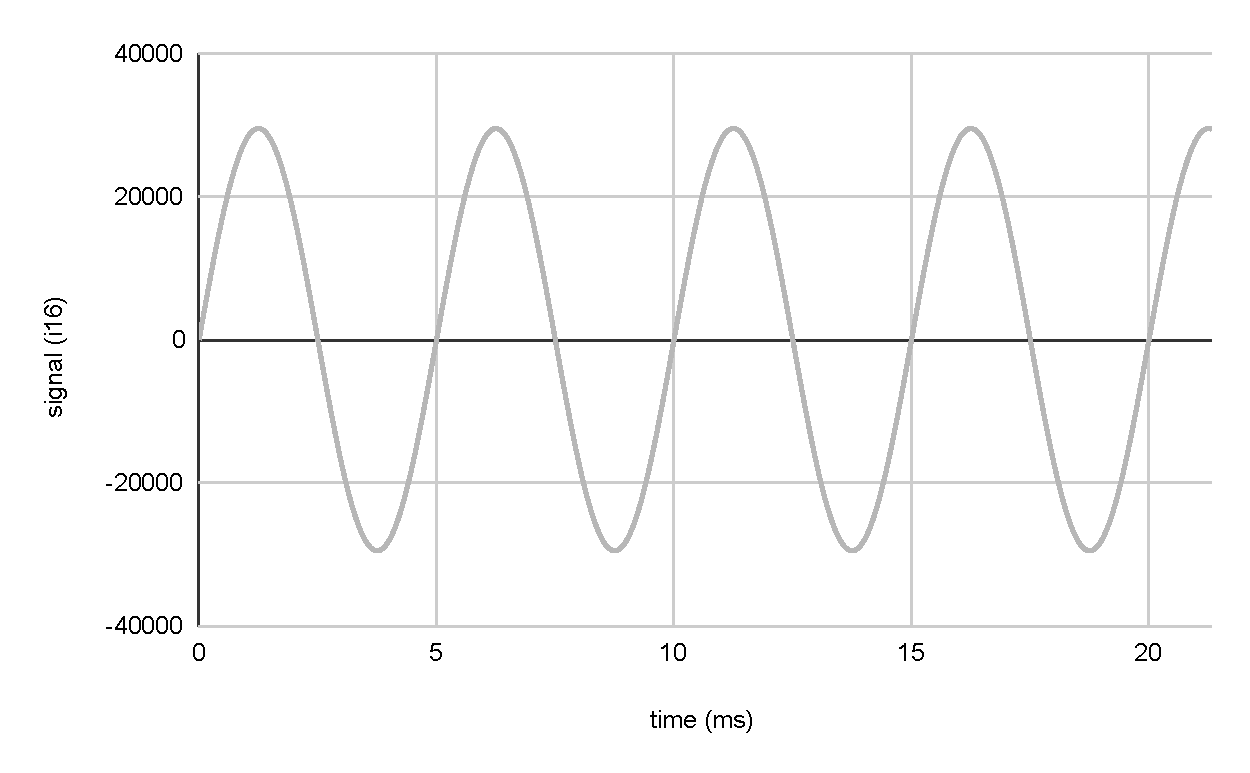
\includegraphics[width=.8\linewidth]{./images/signal_i16.pdf}
        \caption{Signal sinusoïdal à \SI{440}{\hertz} codé en \emph{fixed point} (Q15)}
        \label{fig:signal_i16}
    \end{figure}

    \paragraph{}
    La représentation graphique du spectre de fréquences généré par la MDCT de référence en \emph{fixed point} à partir du signal à \SI{440}{\hertz} est présentée par la figure \ref{fig:validation_ref_mdct_int} :
    \begin{itemize}
        \item le spectre prend la même forme que le spectre de fréquence généré par les MDCT en \emph{floating point} (figure \ref{fig:validation_ref_mdct_float});
        \item le spectre met bien en évidence une composante fréquentielle principale aux alentours de \SI{440}{\hertz};
        \item les valeurs des composantes fréquentielles sont beaucoup plus grandes que celles du spectre en \emph{floating point} puisqu'elles sont mise à échelle Q15.
    \end{itemize}

    \begin{figure}[H]
        \centering
        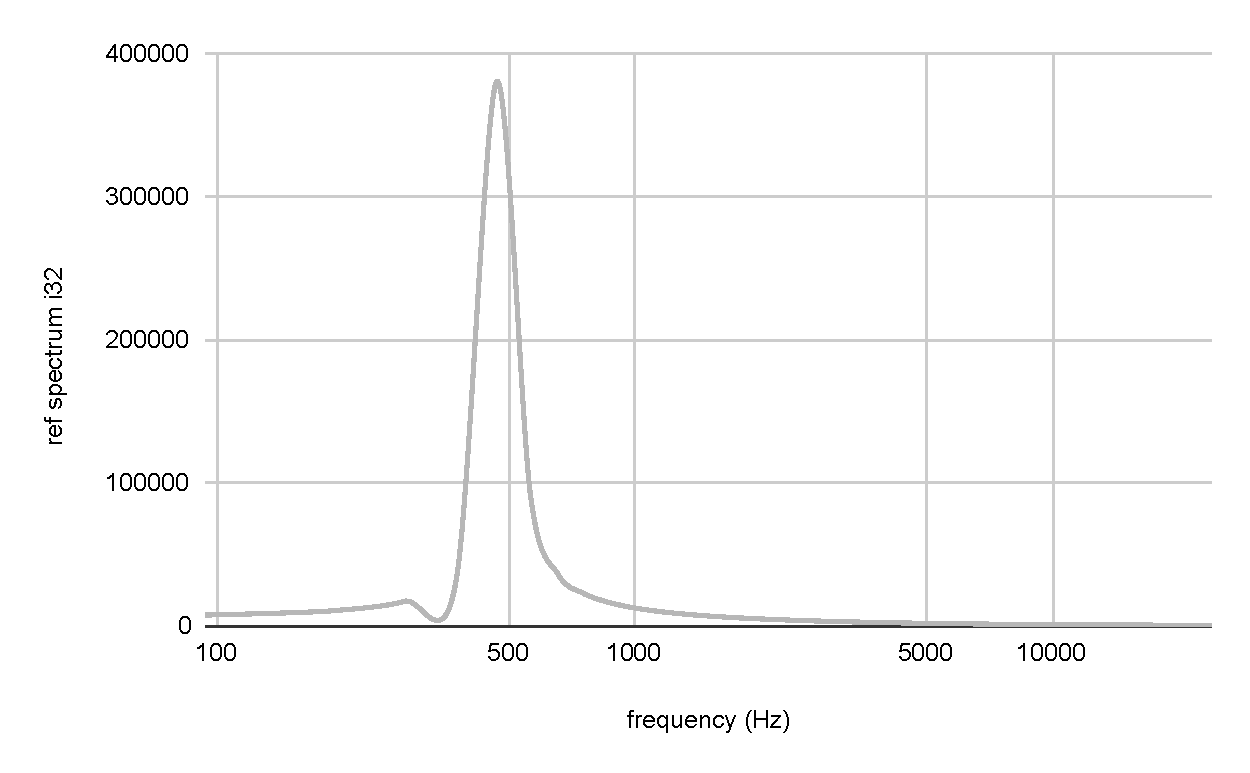
\includegraphics[width=.8\linewidth]{./images/validation_ref_int.pdf}
        \caption{Spectre de fréquences généré par les MDCT de référence en \emph{fixed point}}
        \label{fig:validation_ref_mdct_int}
    \end{figure}


    \newpage
    \section{Algorithme MDCT basé sur la FFT}
    \subsection{Optimisations attendues}
    % algo qui vient du code d'exemple dsprelated, basé sur la FFT
%    \url{https://infoscience.epfl.ch/record/59946}
%    \url{https://www.cis.rit.edu/class/simg716/Gauss_History_FFT.pdf}
%    \url{https://sci-hub.se/https://www.jstor.org/stable/29775194#}

    %jouer sur la symétrie pour ne calculer que la moitié

    % \subsection{Code DSP related}
    % Code qui se base sur une FFT avec opérations de pre et de post twiddle
    % Annexes : code de la MDCT, test et procédure d'installation de la librairie FFTW

    % au code de base, il faut aussi ajouter la fonction de fenêtre (MLT) qui n'était pas présente.
    
    
    % \paragraph{}
    % Choix de l'optimisation de la MDCT basé sur sur une DCT : la FFT -> complexité de O (N log N) (N taille de la fenetre) + O(N) opérations de pré et de post processing.

    % \paragraph{}
    % But : utiliser une FFT déjà optimisée pour n'avoir à optimiser "que" les opérations de pré et de post processing
    % Exemple trouvé sur le site DSP related -> Annexe ? Citation ?

    \subsection{Implémentation de la MDCT basée sur la FFT de la librairie FFTW3}
    % \paragraph{}
    % Code développé à partir de cet exemple en annexe. Il est basé sur la librairie FFTW3 qu'on ne peut pas garder car ne permet pas de travailler en integer -> sera amené à être retravaillé.

    % \paragraph{}
    % Explications des paramètres du code :
    % \begin{itemize}
    %     \item fenêtre de 1024
    %     \item pre-twiddle -> 256
    %     \item FFT => FFT avec une fenêtre d'entrée réduite et donc une complexité réduite
    %     \item post-twiddle -> 512
    % \end{itemize}

    % \subsection{Réduction de la fenêtre d'entrée}
    % (pre et post processing/twiddles pour faire moins de FFT) -> réduction de la fenêtre de la FFT

    \subsection{Validation}
    % \paragraph{}
    % Validé avec un single tone signal + l'algo de référence.

    \paragraph{}% TODO
    % Présentation des résultats sous forme de données brutes ou de graphique.
    \begin{figure}[H]
        \centering
        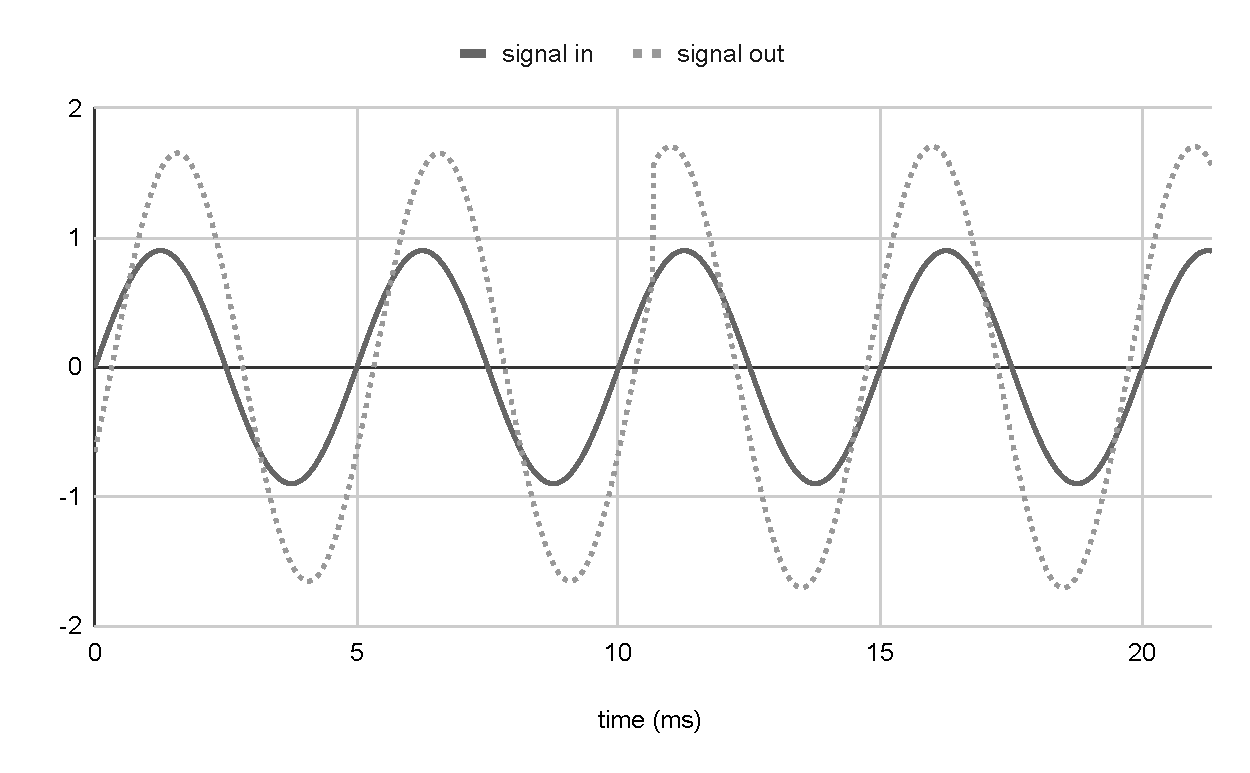
\includegraphics[width=.8\linewidth]{./images/fftw3_mdct_f32_signal_in_out.pdf}
        \caption{Signaux temporels en entrée de la MDCT FFTW3 \emph{float} et en sortie de la IMDCT}
        \label{fig:signal_imdct}
    \end{figure}


    % \paragraph{}
    % Code d'exemple qui teste l'algo de référence et l'algo FFTW3 avec les mêmes données d'entrée pour comparaison. (on fait la différence pour la précision ? ce n'est peut être pas pertinent de la faire déjà)

    % \paragraph{}
    % Présentation des résultats sous forme de données brutes ou de graphiques.

    % A ce niveau, pour valider, j'ai aussi essayé de faire la IMDCT mais dû à l'overlap, sur une seule fenetre, on ne sait pas reconstruire le signal -> pas possible de valider comme ça

    \begin{figure}[H]
        \centering
        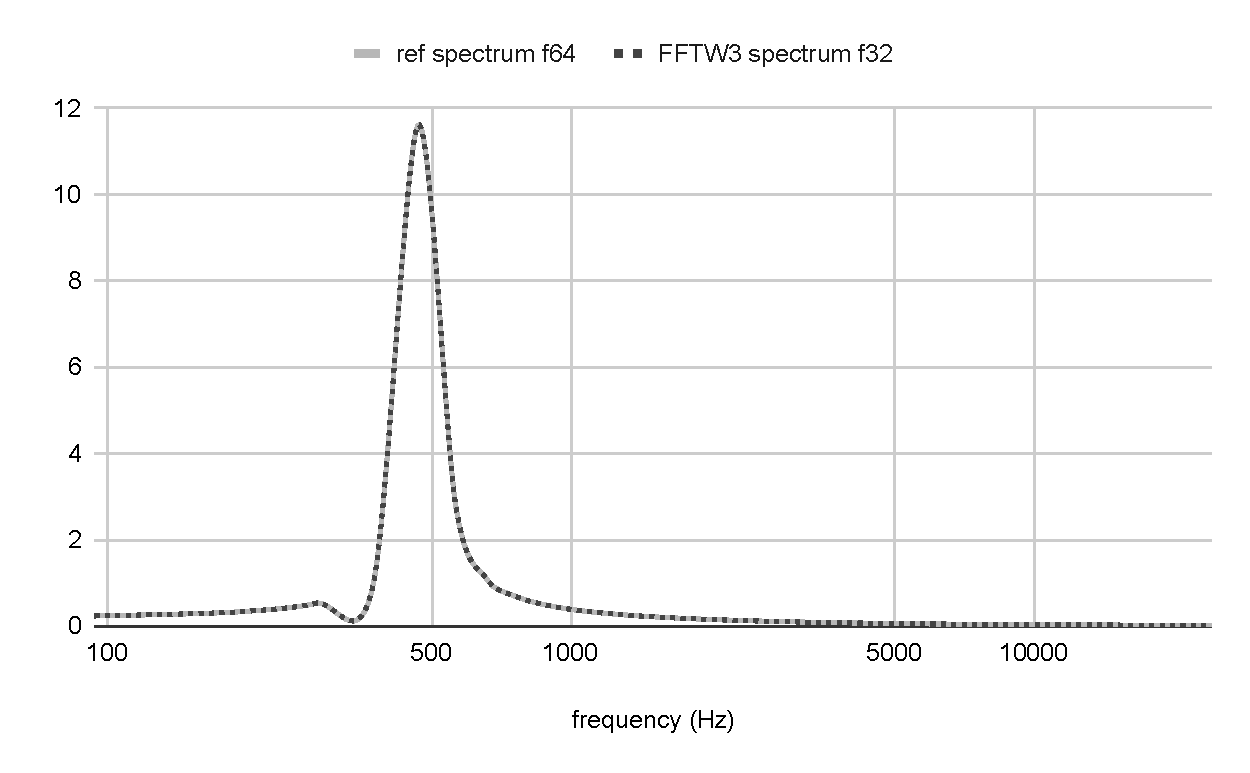
\includegraphics[width=.8\linewidth]{./images/validation_fftw_f32.pdf}
        \caption{Spectre de fréquences généré par la MDCT FFTW3 \emph{float} comparé au spectre de référence}
        \label{fig:validation_fftw3_f32}
    \end{figure}


    \newpage
    \section{Intégration de la librairie \emph{Ne10}}
    \subsection{Choix de la librairie}
    \paragraph{}
    La librairie \emph{FFTW3} utilisée pour l'itération précédente de la MDCT ne propose pas de FFT en algorithmique entière. Le passage à une autre librairie était donc nécessaire et le choix s'est porté sur la librairie \emph{Ne10} qui propose différentes FFT en \emph{fixed point}.

    \paragraph{}
    Le projet \emph{Ne10} propose toute une série de fonctions mathématiques et physiques de base ainsi que des fonctions de traitement de signal et de traitement d'image. La librairie est spécifiquement développée pour les architectures ARM possédant les opérations SIMD Neon (ARMv7 et ARMv8-A)\cite{Ne10}.

    \paragraph{}
    \emph{Ne10} propose à la fois des fonctions développées en \emph{plain C} et des fonctions optimisées avec les instructions SIMD Neon : les deux types de fonctions seront utilisées pour développer une MDCT optimisée et pour conserver une MDCT de référence en \emph{plain C}. Maintenir une MDCT \emph{plain C} permettra d'avoir une référence pour la mesure des performances de l'algorithme \emph{fixed point} mais pourrait aussi s'avérer utile pour une utilisation de l'encodeur AAC sur une architecture ARM ne possédant pas les instructions Neon.

    \paragraph{}
    L'utilisation de la librairie \emph{Ne10} est soumise à la licence \emph{3-Clause BSD}, license permissive qui permet un usage commercial des produits intégrant la librairie et qui ne contraint pas à en distribuer le code source\cite{BSD}.

    \subsection{Implémentation de la MDCT basée sur la FFT \emph{Ne10} en \emph{float 32}}
    \paragraph{}
    La librairie \emph{Ne10} s'installe simplement en suivant les instructions données par la documentation : clone du projet GitHub, run du CMake et build du projet\cite{Ne10}. La librairie ne peut cependant être installée que sur une plateforme Linux, Android ou iOS reposant sur une architecture ARM. À partir de ce moment, il n'est donc plus possible de maintenir une implémentation de référence de la MDCT pour une architecture Intel.

    \paragraph{}
    \emph{Ne10} propose des algorithmes de FFT \emph{real to complex} et \emph{complex to complex} en \emph{floating point} (32 bits) ou en \emph{integer} (32 bits et 16 bits). L'objectif est évidemment de passer toute la MDCT en \emph{integer} mais pour un premier test de la librairie, l'algorithme de la section précédente a tout d'abord été repris en remplaçant la FFT de \emph{FFTW3} par la fonction \texttt{ne10\_fft\_c2c\_1d\_float32\_neon} de \emph{Ne10} : FFT en \emph{complex to complex} en \emph{float 32}, i.e. l'entrée et la sortie de la FFT sont représentées sous forme de tableaux de nombres complexes codés en \emph{float} sur 32 bits.

    \paragraph{}
    L'annexe \ref{an:mdct_ne10_f32} présente le code de cette implémentation. L'annexe \ref{an:mdct_ne10_f32_header} montre que ce code est construit sur le même modèle que le code utilisant la librairie \emph{FFTW3}. La classe contient la configuration de la FFT et les tableaux contenant les données d'entrée, les données de sortie et les facteurs de twiddling. La classe définit trois fonctions publiques : le constructeur, le destructeur et la fonction MDCT.

    \paragraph{}
    L'annexe \ref{an:mdct_ne10_f32_constructor} montre l'initialisation de la MDCT dans le constructeur de la classe. Le constructeur initialise les tableaux de facteurs de twiddling de le même manière que l'algorithme basé sur la FFT de \emph{FFTW3}. La configuration de la FFT de \emph{Ne10} se fait conformément au code d'exemple donné par la documentation de la librairie\cite{Ne10} avec en paramètre la taille de la FFT qui correspond au quart de la taille de la fenêtre d'entrée.

    \paragraph{}
    Le destructeur présenté à l'annexe \ref{an:mdct_ne10_f32_destructor} permet de libérer la mémoire allouée pour la FFT en appelant la fonction adéquate de la librairie \emph{Ne10}.

    \paragraph{}
    La fonction MDCT présentée dans l'annexe \ref{an:mdct_ne10_f32_func}, comme pour l'algorithme précédent :
    \begin{itemize}
        \item effectue les opérations de \emph{pre-processing} ou \emph{pre-twiddling} : ce sont les mêmes que celle de la MDCT \emph{FFTW3} en arithmétique \emph{floating point} sur 32 bits;
        \item appelle l'algorithme de FFT : la FFT de \emph{Ne10} prend en paramètres les tableaux contenant les données d'entrée et de sortie, la configuration de la FFT et un \emph{integer} à \texttt{0} pour réaliser la FFT ou à \texttt{1} pour réaliser l'opération inverse;
        \item effectue les opérations de \emph{post-processing} ou \emph{post-twiddling} : ici aussi les mêmes que celles de la MDCT \emph{FFTW3} en arithmétique \emph{floating point} sur 32 bits.
    \end{itemize}

    \paragraph{}
    L'algorithme développé ici ne diffère donc pas de l'algorithme présenté à la section précédente. Son développement est trivial mais il permet de tester et de valider le fonctionnement de la librairie \emph{Ne10}.

    \subsection{Validation}
    \paragraph{}
    L'utilisation de la librairie \emph{Ne10} est validée par comparaison du spectre de fréquences qu'elle génère avec les spectres générés par la MDCT de référence en \emph{double} et par la MDCT basée sur \emph{FFTW3} également en \emph{double}. Les MDCT sont appelées en \emph{double} pour plus de précision. La comparaison aurait pu se faire sur base de tous les algorithmes de MDCT en \emph{float} sur 32 bits mais le choix qui a été fait ici permet en plus de vérifier que la perte de précision entre le \emph{float} et le \emph{double} soit acceptable.

    \paragraph{}
    Le code source permettant de comparer les trois MDCT en \emph{floating point} est présenté à l'annexe \ref{an:valid_comp_source}. Il sera expliqué en détail dans la section \ref{sec:validation} consacrée à la validation des données des MDCT. Compilé avec les commandes CMake de l'annexe \ref{an:valid_comp_float}, le code produit un exécutable permettant de comparer les spectres de fréquence produits par les trois MDCT \emph{floating point} en les affichant en console.

    \begin{figure}[H]
        \centering
        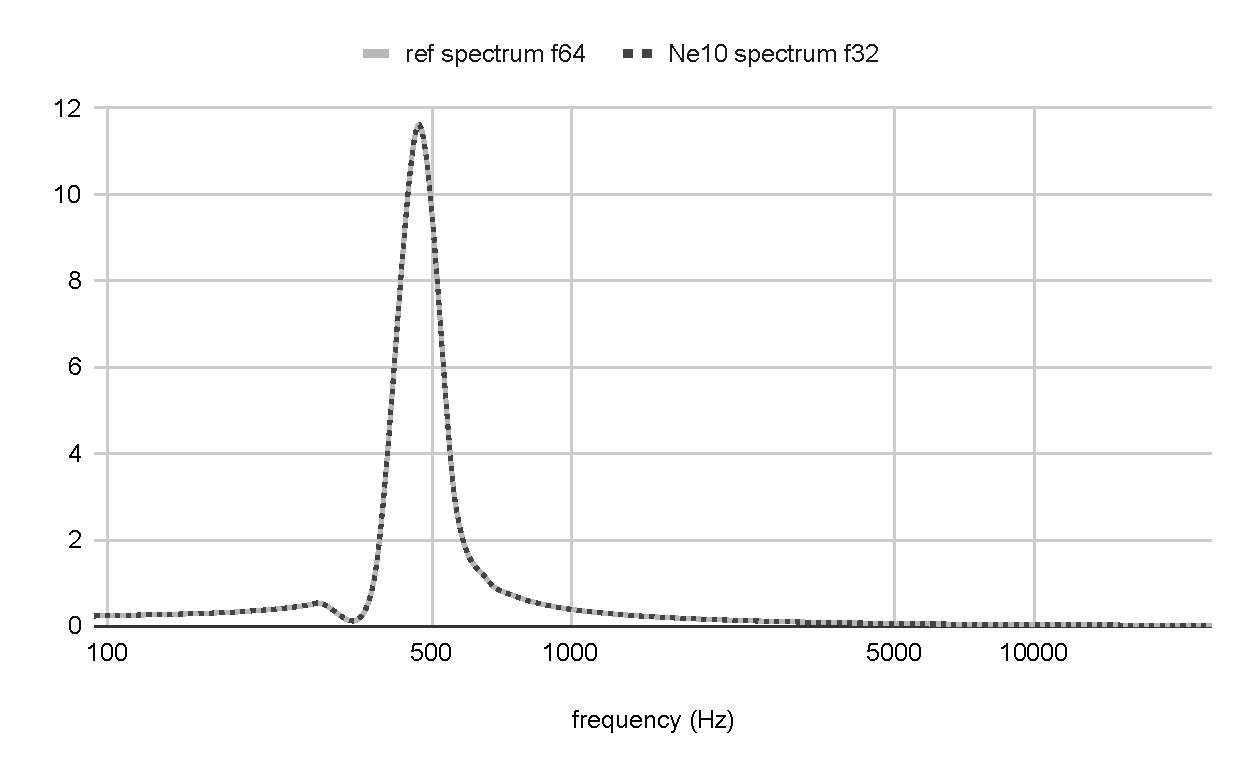
\includegraphics[width=.8\linewidth]{./images/validation_ne10_f32.pdf}
        \caption{Spectre de fréquences généré par la MDCT Ne10 i32 plain C comparé au spectre de référence}
        \label{fig:validation_ne10_f32}
    \end{figure}

    \paragraph{}
    En redirigeant les données sorties en console vers un fichier texte, il est possible d'exploiter ces données sous forme de graphique. (voir figure \ref{fig:comp_mdct_float}) TODO : explication du graphique

    \paragraph{}
    TODO : présentation de la précision

    \subsection{Performances}
    \label{sec:fft_perfs}
    Une fois l'utilisation de la librairie \emph{Ne10} validée,  Mesure de la différence de performance entre différentes FFT : code en annexe

    FFT Ne10 f32 plain C
    average run time:   5632.06 ns
    standard deviation: 4.38439e-09 ns

    FFT Ne10 f32 Neon
    average run time:   3115.18 ns
    standard deviation: 2.81769e-06 ns

    FFT Ne10 i32 plain C
    average run time:   10723.1 ns
    standard deviation: 1.77145e-06 ns

    FFT Ne10 i32 Neon
    average run time:   3455.78 ns
    standard deviation: 5.35823e-07 ns

    FFT Ne10 i16 plain C
    average run time:   9557.52 ns
    standard deviation: 1.69145e-07 ns

    FFT Ne10 i16 Neon
%     average run time:   2007.07 ns
%     standard deviation: 2.58836e-07 ns
% 
%     FFT FFTW3 f32 plain C
%     average run time:   4641.64 ns
%     standard deviation: 2.69836e-07 ns
% 
%     echo "Ne10 FFT f32 plain C"
%     ./../build/audio_encoding/run_ne10_fft_f32_c
%     
%     echo "Ne10 FFT i32 plain C"
%     ./../build/audio_encoding/run_ne10_fft_i32_c
%     
%     echo "Ne10 FFT i16 plain C"
%     ./../build/audio_encoding/run_ne10_fft_i16_c
%     
%     echo "Ne10 FFT f32 neon"
%     ./../build/audio_encoding/run_ne10_fft_f32_neon
%     
%     echo "Ne10 FFT i32 neon"
%     ./../build/audio_encoding/run_ne10_fft_i32_neon
%     
%     echo "Ne10 FFT i16 neon"
%     ./../build/audio_encoding/run_ne10_fft_i16_neon
%     
%     echo "FFTW3 FFT f32 plain C"
%     ./../build/audio_encoding/run_fftw3_fft_f32
% 
%     ./audio_encoding/run_fftw3_mdct_f32 
% MDCT FFTW3 f32 plain C: 10000000 runs with a single tone signal (440Hz)
% average run time: 7599.66 ns
% standard deviation: 2.06124e-06
% pi@rpi-evs-dev01:~/Dev/aac-lbin/build $ ^C
% pi@rpi-evs-dev01:~/Dev/aac-lbin/build $ cd ../
% algorithms/     build/          .git/           wav/            
% audio_encoding/ fftw-3.3.9/     Ne10/           
% pi@rpi-evs-dev01:~/Dev/aac-lbin/build $ cd ../audio_encoding/
% pi@rpi-evs-dev01:~/Dev/aac-lbin/audio_encoding $ ./test/performance/mdct_performance.sh 
% MDCT Ne10 i32 C
% MDCT Ne10 i32 plain C: 1000000 runs with a single tone signal (440Hz)
% average run time: 14918.7 ns
% standard deviation: 2.0867e-07
% MDCT Ne10 i32 Neon
% MDCT Ne10 i32 Neon: 1000000 runs with a single tone signal (440Hz)
% average run time: 5804.49 ns
% standard deviation: 1.37386e-08
% MDCT Ne10 f32 C
% MDCT Ne10 f32 plain C: 1000000 runs with a single tone signal (440Hz)
% average run time: 8920.73 ns
% standard deviation: 3.7541e-10
% FFTW3 MDCT f32
% MDCT FFTW3 f32 plain C: 10000000 runs with a single tone signal (440Hz)
% average run time: 7584.66 ns
% standard deviation: 1.66076e-07
% pi@rpi-evs-dev01:~/Dev/aac-lbin/audio_encoding \$ ./test/performance/fft_performance.sh 
% Ne10 FFT f32 plain C
% FFT Ne10 f32 plain C
% average run time:   5538.36 ns
% standard deviation: 6.1161e-07 ns
% Ne10 FFT i32 plain C
% FFT Ne10 i32 plain C
% average run time:   10678.9 ns
% standard deviation: 2.126e-06 ns
% Ne10 FFT i16 plain C
% FFT Ne10 i16 plain C
% average run time:   9569.07 ns
% standard deviation: 1.58159e-08 ns
% Ne10 FFT f32 neon
% FFT Ne10 f32 Neon
% average run time:   3013.71 ns
% standard deviation: 1.18327e-07 ns
% Ne10 FFT i32 neon
% FFT Ne10 i32 Neon
% average run time:   3396.91 ns
% standard deviation: 8.48083e-07 ns
% Ne10 FFT i16 neon
% FFT Ne10 i16 Neon
% average run time:   2002.41 ns
% standard deviation: 8.582e-08 ns
% FFTW3 FFT f32 plain C
% FFT FFTW3 f32 plain C
% average run time:   4661.46 ns
% standard deviation: 1.36369e-07 ns



    \newpage
    \section{Algorithme MDCT en arithmétique fixed point}
    \label{sec:fixed_point}
    \paragraph{}
    Le passage d'une arithmétique flottante à une arithmétique entière est une des optimisations envisagées par l'analyse préalable à ce travail. Le bénéfice attendu est double : l'arithmétique entière est généralement plus rapide et un bloc MDCT en arithmétique entière serait mieux intégré à l'ensemble de l'encodeur.

    \paragraph{}
    La première de ces attentes n'a pas pu être rencontrée. En effet, l'architecture ARMv7 du Raspberry supporte de nombreuses instructions en \emph{floating point} sur 32 bits\cite{DOC-ARM}. Or, plusieurs instructions \emph{fixed point} sont souvent nécessaires pour remplacer une seule instruction en \emph{floating point}, e.g. une multiplication en float est remplacée au minimum par une multiplication et une rotation de bits pour que le produit tienne sur le même nombre de bits que les nombres multipliés. Plutôt que de gagner en temps d'exécution, le passage en \emph{fixed point} a ralenti la MDCT.

    \paragraph{}
    Cependant, le passage en \emph{fixed point} permet d'économiser un transtypage du \emph{integer} vers le \emph{float} en entrée de la MDCT et inversement en sortie. Avec un temps d'exécution au moins équivalent en \emph{fixed point} qu'en \emph{floating point}, le passage en \emph{fixed point} permettrait donc tout de même d'améliorer les performances de l'ensemble de l'encodeur AAC.

    \paragraph{}
    Enfin, les données reçues à l'entrée de la MDCT sont codées en \emph{integer} sur 16 bits alors que les \emph{float} sont codés au minimum sur 32 bits. Garder le maximum de données et d'opérations en 16 bits permettrait de gagner en performance au moment de l'utilisation des opérations SIMD.

    \subsection{Arithmétique fixed point}

    \paragraph{}
    La représentation \emph{fixed point} est une alternative au \emph{float} pour le codage des nombres décimaux\cite{2007-Oberstar}. Le principe est de réserver un certain nombres de bits pour coder la partie entière et un autre nombre de bits pour coder la partie décimale du nombre. Ce travail utilise deux notations pour la représentation en \emph{fixed point}, toujours signée :
    \begin{itemize}
        \item $Qm$ où $m$ est le nombre de bits réservés aux décimales, e.g. une notation Q15 sur 16 bits permet de représenter un nombre signé ne contenant que des décimales et pas de partie entière puisqu'un bit est réservé pour le signe;
        \item $Qx.y$ où $x$ est le nombre de bits réservés à la partie entière et $y$ le nombre de bits réservés à la partie décimale, e.g. une notation Q1.15 équivaut à une notation Q15 sur 16 bits.
    \end{itemize}

    \paragraph{}
    Pour passer la MDCT en algorithmique \emph{fixed point}, il faut tout d'abord prêter attention à choisir la représentation adéquate. Par exemple, les données d'entrée de la MDCT sont comprises entre $0.9$ et $-0.9$. Elles peuvent donc être représentées en Q15. Si elles avaient été comprises ente $1$ et $-1$, la conversion à une représentation Q15 aurait produit un dépassement sur l'une des valeurs limites et par conséquent une perte d'information.

    \paragraph{}
    Des dépassements peuvent également se produire lors des opérations arithmétiques :
    \begin{itemize}
        \item une \textbf{addition} ou une \textbf{soustraction} peut causer un dépassement d'un bit, e.g. la somme d'un nombre sur 32 bits et d'un nombre sur 16 bits nécessite potentiellement 33 bits pour être codée;
        \item le résultat d'une \textbf{multiplication} ou d'une \textbf{division} peut devoir être codé sur un nombre de bits équivalent à la somme des nombres de bits composants les deux nombres multipliés ou divisés, e.g. le produit d'un nombre de 16 bits multiplié par un nombre de 32 bits nécessite potentiellement 48 bits pour être codé.
    \end{itemize}

    \paragraph{}
    Ces dépassements sont théoriques. En fonction des données réelles à traiter, il est possible de ne pas respecter à la lettre les règles énoncées plus haut. C'est le cas par exemple avec les facteurs de \emph{twiddling} dont on sait qu'il valent au maximum un quart de la valeur d'un sinus ou d'un cosinus et qui sont codés en Q15 : il est alors certain que l'addition de deux de ces nombres ne causera pas de dépassement.

    \paragraph{}
    Là où l'implémentation en \emph{floating point} était triviale, puisqu'elle demandait simplement de reprendre le code d'exemple fourni et de l'adapter à l'utilisation de la librairie \emph{Ne10}, l'implémentation en \emph{fixed point} devient plus complexe : il faut prêter attention à coder les nombres dans les bonnes ranges et implémenter les différentes opérations arithmétiques de sorte à ne pas causer de dépassements.

    \subsection{Implémentation de la MDCT basée sur la FFT Ne10 en arithmétique \emph{fixed point}}
    \label{sec:ne10_mdct_i32_c}
    \paragraph{}
    L'\textbf{annexe J} présente l'implémentation de la MDCT \emph{Ne10 fixed point} en \emph{plain C}. La classe \texttt{mdct\_ne10\_i32\_c} a la même structure que l'implémentation en \emph{floating point}. Le header présenté dans l'\textbf{annexe J.1} montre que seul le type des données a changé :
    \begin{itemize}
        \item La configuration et les tableaux d'entrée et de sortie de la FFT sont définis avec les types \texttt{int32}, et non plus \texttt{float32}, de la librairie \emph{Ne10};
        \item Le tableau de facteurs de \emph{twiddling} passe du \texttt{float} au \texttt{int16\_t};
        \item La fonction MDCT prend en paramètres un signal temporel en \texttt{int16\_t} et renvoie un spectre en \texttt{int32\_t} au lieu des tableaux de \texttt{float}.
    \end{itemize}

    \subsubsection{Utilisation de la FFT \emph{Ne10} en \emph{int 32}}
    \paragraph{}
    L'utilisation de la librairie \emph{Ne10} en \emph{integer} est très peu différente de son utilisation en \emph{float} :
    \begin{itemize}
        \item La configuration est initialisée dans le constructeur de la classe \texttt{mdct\_ne10\_i32\_c} (\textbf{annexe J.2}) en \emph{complex to complex} en \emph{integer 32} avec en paramètre la taille de la fenêtre de la FFT réduite à un quart de la taille de la fenêtre d'entrée.
        \item L'espace alloué à la configuration est libéré dans le destructeur de la classe \texttt{mdct\_ne10\_i32\_c} (\textbf{annexe J.3}) avec la fonction appropriée de la librairie \emph{Ne10};
        \item La fonction de FFT est appelée avec en paramètres le tableau contenant les données d'entrée, le tableau dans lequel sera calculé le résultat de la FFT, la configuration préalablement initialisée, un \emph{integer} qui indique à la fonction de réaliser la FFT et non son opération inverse et, en plus de la FFT en \emph{float}, un facteur de mise à échelle mis ici à $0$.
    \end{itemize}

    \paragraph{}
    Il est à noter que l'initialisation du facteur de mise à échelle de la fonction de FFT n'est pas documentée dans la librairie \emph{Ne10}. L'effet de ce facteur sur la FFT n'est pas non plus indiqué. J'ai initialisé ce facteur à 0 après avoir testé la FFT de \emph{Ne10} dans le but d'obtenir les mêmes valeurs qu'en \emph{float} mises à une échelle Q15.

    \paragraph{}
    La documentation incomplète de la librairie a été une des difficultés de ce travail. En dehors des quelques codes d'exemples disponibles, il est très compliqué de savoir quelles données sont attendues et sont produites par les fonctions de \emph{Ne10}. Il est également très difficile de trouver des ressources externes sur l'utilisation de \emph{Ne10}.

    \paragraph{}
    % TODO dire que ni moi ni les autres n'avons trouvé comment faire
    Le manque de documentation est également ce qui a empêché l'utilisation de la FFT en \emph{int16} plutôt qu'en \emph{int32}. Des opérations en 16 bits pour tout le bloc MDCT auraient été plus performantes. Malheureusement, si la documentation de \emph{Ne10} dit bien travailler en Q15 pour du 16 bits et en Q31 pour du 32 bits, elle ne dit pas quelle \emph{headroom} prévoir, quelles \emph{ranges} de valeurs sont acceptées, si les opérations saturent ou non, etc. En testant la FFT 16 bits avec des données codées en Q15, trop de valeurs fausses étaient produites par la FFT. L'utilisation du facteur de mise à échelle n'a pas non plus permis d'obtenir de résultats satisfaisant.

    \paragraph{}
    Pour ne pas produire de dépassement dans la fonction de FFT, il a fallu prévoir 8 bits de \emph{headroom} pour la FFT. Sur des données codées sur 16 bits, cela signifie qu'il ne resterait plus que 8 bits de données utiles pour le signal, dont 1 bit pour le signe. Cette perte de précision trop importante a forcé l'utilisation de la FFT en 32 bits.


    \subsubsection{Initialisation des \emph{twiddle factors}}
    \paragraph{}
    Le tableau de facteurs de \texttt{twiddle} est initialisé dans le constructeur de la classe \texttt{mdct\_ne10\_i32\_c} (\textbf{annexe J.2}). Ses valeurs sont calculées en \emph{double} puis converties en \emph{integer} (représentation Q15).
    
    \paragraph{}
    Il aurait été posible de convertir les opérations d'initialisation en \emph{fixed point} mais l'optimisation du constructeur n'est pas nécessaire. En effet, puisque la taille de fenêtre d'entrée ne varie pas, l'appel de l'initialisation ne sera fait qu'une fois et la MDCT est ensuite appelée en boucle avec les mêmes facteurs de \emph{twiddling}.

    \subsubsection{Opérations de \emph{pre-twiddling} et de \emph{post-twiddling}}
    \paragraph{}
    L'essentiel du tavail pour cette implémentation a été le passage des opérations de \emph{pre-} et de \emph{post-processing} en arithmétique \emph{fixed point}. Le résultat de ce travail est présenté dans l'\textbf{annexe J.3} qui présente la fonction MDCT basée sur la FFT de \emph{Ne10} en \emph{plain C}.

    \paragraph{}
    Les opérations de \emph{pre-twiddling} transforment le signal temporel et les facteurs de \emph{twiddling}, tous deux en représentation Q15, en un nombre en représentation Q1.23 sur 32 bits à donner en entrée de la FFT de \emph{Ne10} en \emph{int32}. La représentation Q1.23 est celle qui permet de garder le maximum de précision tout en s'assurant de ne pas produire de dépassement dans la FFT en gardant 8 bits de \emph{headroom}.

    \paragraph{}
    Le \emph{post-twiddling} récupère les données en Q9.23 produites par la FFT de \emph{Ne10} : la précision de 23 décimales donnée en entrée, le bit de signe et les 8 bits de \emph{headroom}. En combinaison avec les facteurs de \emph{twiddling} codés en Q15, elles sont transformées en un spectre de fréquences codé en Q9.15 sur 32 bits.

    \paragraph{}
    Les opérations de \emph{pre-processing} suivent toujours le même schéma : les parties réelles ou imaginaires des données d'entrée de la FFT sont la somme de deux produits d'un facteur de \emph{twiddling} et de la somme de deux échantillons du signal temporel. Voici en exemple la transformation de la première opération de l'arithmétique \emph{floating point} vers l'arithmétique \emph{fixed point} :
    $$fft\_in[i/2].r = r0*c + i0*s;$$
    $$\text{devient}$$
    $$fft\_in[i/2].r = (((r0*c)+64)>>7) + (((i0*s)+64)>>7);$$
    $$\text{où } r0 = time\_signal[MDCT_M32-1-i] + time\_signal[MDCT_M32+i];$$
    $$\text{et } i0 = time\_signal[MDCT_M2+i] - time\_signal[MDCT_M2-1-i];$$

    \begin{description}
        \item[r0] est la somme de deux échantillons du signal temporel codés en Q1.15 : il correspond donc à une notation \textbf{Q2.15} ici codée sur 32 bits plutôt que de perdre un bit de précision pour garder la valeur sur 16 bits;
        \item[c] \emph{twiddle factor}, est codé en Q1.15, mais on sait que le facteur de mise à échelle pour une fenêtre de 1024 échantillons temporels l'a réduit à $\frac{1}{4}$ de la range possible du Q1.15, noté \textbf{Q1.15/4};
        \item[r0*c] le produit d'un nombre en Q2.15 avec un nombre Q1.15 est théoriquement un Q2.30 mais tient en pratique sur du \textbf{Q1.30/2} puisque le \emph{twiddle factor} est en Q1.15/4;
        \item[((r0*c)+64)>>7] le résultat en Q1.30/2 est ramené à du \textbf{Q1.23/2} par une opération de shift avec arrondi ($64 = 2^6$, ajouter un bit en $7^{\text{ème}}$ position en partant du LSB permet d'arrondir la valeur du $8^{\text{ème}}$ bit);
        \item[((i0*s)+64)>>7] l'opération est équivalente à la précédente et est donc également codée en \textbf{Q1.23/2};
        \item[(((r0*c)+64)>>7) + (((i0*s)+64)>>7)] l'addition de deux Q1.23/2 donne un \textbf{Q1.23}, codé sur 32 bits, il permet de conserver les 8 bits de \emph{headroom} nécessaire à la FFT.
    \end{description}

    \paragraph{}
    Les opérations de \emph{post-processing} suivent elles aussi toujours le même schéma : les valeurs du spectre de fréquences sont calculées en additionnant deux produits d'un facteur de \emph{twiddling} et d'une donnée de sortie de la FFT. Voici en exemple la conversion de la première opération de \emph{post-twiddling} en \emph{fixed point} :
    $$spectrum[i] = -r0*c - i0*s;$$
    $$\text{devient}$$
    $$spectrum[i] = ((((-r0+128)>>8)*c+16384)>>15) - ((((i0+128)>>8)*s+16384)>>15);$$
    $$\text{où } r0 \text{ et } i0 \text{ sont les parties réelle et imaginaire des données de sortie de la FFT}$$

    \begin{description}
        \item[r0] donnée de sortie de la FFT, est codé en \textbf{Q9.23};
        \item[(-r0+128)>>8] $r0$ est ramené en \textbf{Q9.15} par un \emph{shift} de 8 avec arrondi;
        \item[c] \emph{twiddle factor}, est codé en Q1.15, mais on sait que le facteur de mise à échelle pour une fenêtre de 1024 échantillons temporels l'a réduit à $\frac{1}{4}$ de la range possible du Q1.15, noté \textbf{Q1.15/4};
        \item[((-r0+128)>>8)*c] la multiplication d'un Q9.15 par un Q1.15/4 donne un Q10.30/4 ou \textbf{Q9.30/2};
        \item[(((-r0+128)>>8)*c+16384)>>15] le résultat en Q9.30/2 est ramené à du \textbf{Q9.15/2} par un \emph{shift} de 15 avec arrondi;
        \item[(((i0+128)>>8)*s+16384)>>15] le second terme effectue les mêmes opérations pour un résultat en \textbf{Q9.15/2};
        \item[((((-r0+128)>>8)*c+16384)>>15) - ((((i0+128)>>8)*s+16384)>>15)] la différence de deux Q9.15/2 est un Q10.15/2 ou \textbf{Q9.15}.
    \end{description}


    \subsection{Validation}
    \paragraph{}
    L'algorithme est validé par comparaison avec l'algorithme de référence. Le protocole de validation est détaillé dans la section \ref{sec:validation} : les spectres sont générés par les différentes MDCT sur base du même signal temoprel pour que tous les spectres puissent être comparés entre eux. Afin de s'assurer de la cohérence des données produites par la MDCT, le signal d'entrée est un signal sinusoïdal : le spectre de fréquences ne doit donc mettre en évidence qu'une seule composante fréquentielle.

    \paragraph{}
    La figure \ref{fig:validation_ne10_i32_c} montre la comparaison entre le spectre de fréquences généré par la MDCT basée sur la FFT Ne10 en plain C et celui de référence en \emph{integer} sur 32 bits (calculs en \emph{double} mis à échalle Q15) pour un signal d'entrée à \SI{200}{\hertz}.

    \begin{figure}[H]
        \centering
        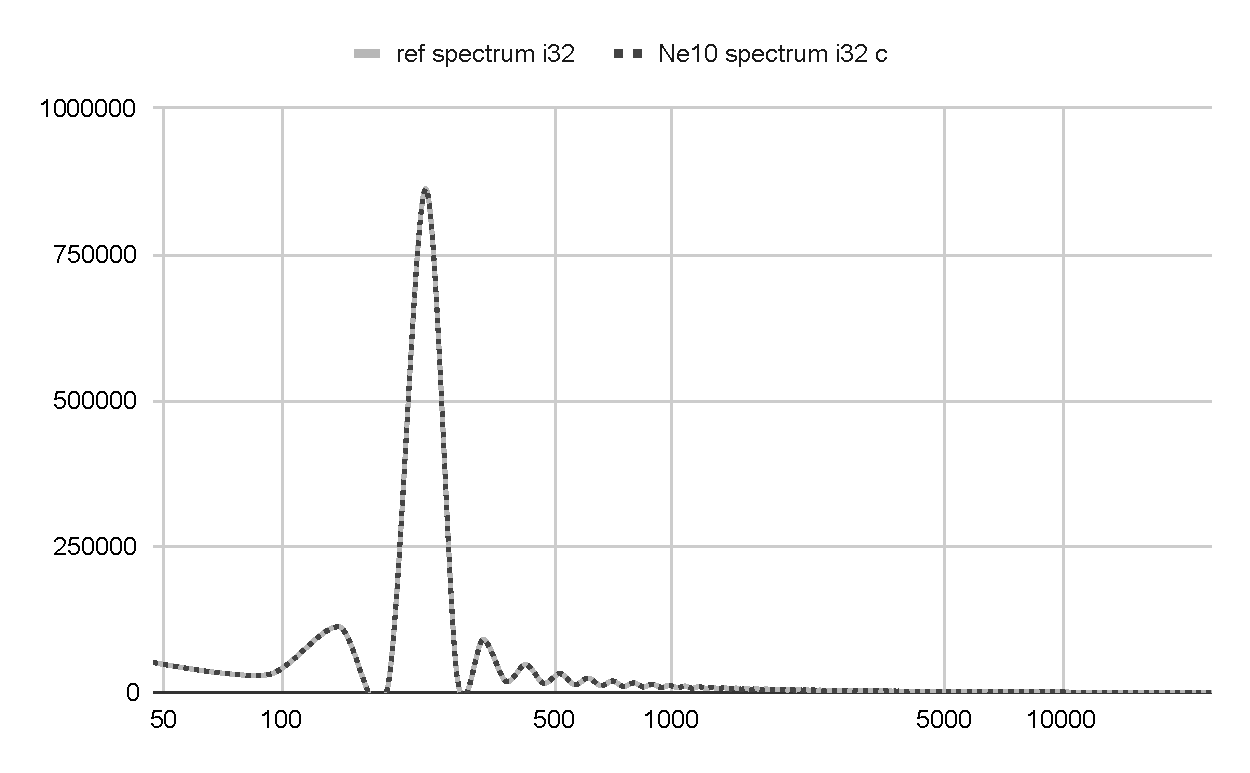
\includegraphics[width=.8\linewidth]{./images/validation_ne10_i32_c.pdf}
        \caption{Spectre de fréquences généré par la MDCT Ne10 i32 plain C comparé au spectre de référence}
        \label{fig:validation_ne10_i32_c}
    \end{figure}

    \paragraph{}
    Le spectre de fréquences généré par la MDCT Ne10 i32 plain C (en pointillés) se superpose presque parfaitement au spectre de référence. La composante fréquentielle la plus haute se situe bien aux alentours de \SI{200}{\hertz}.

    % TODO precision ?


    \subsection{Performances}
    \label{sec:fixed_point_perfs}
    \paragraph{}
    Les performances de la MDCT \emph{fixed point} en \emph{plain C} sont moins bonnes que celles de l'implémentation en \emph{floating point} (voir section \ref{sec:mdct_perfs} pour plus d'explications sur la mesure des performances):
    \begin{itemize}
        \item La MDCT \emph{Neon float 32 plain C} a un temps d'exécution moyen de \SI{9}{\micro\second};
        \item La MDCT \emph{Neon integer 32 plain C} a un temps d'exécution moyen de \SI{22}{\micro\second}.
    \end{itemize}

    \paragraph{}
    Le temps d'exécution notablement plus conséquent s'explique par le fait que l'architecture ARMv7 supporte de nombreuses opérations \emph{floating point} sur 32 bits. Contrairement à des processeurs plus anciens, l'ARMv7 n'est donc pas plus efficace en arithmétique \emph{fixed point}.

    \paragraph{}
    De plus, la section \ref{sec:ne10_mdct_i32_c} a montré qu'une seule instruction en \emph{floating point} était remplacée par plusieurs opérations \emph{fixed point}. Une multiplication est, par exemple, remplacée par une multiplication, une rotation et une addition pour l'arrondi. Puisque les opérations sur des \emph{integer} ne sont pas plus rapides que sur des \emph{float}, il n'est donc pas étonnant que la MDCT \emph{fixed point} soit plus lente que la MDCT \emph{floating point}.

    \paragraph{}
    L'algorithme \emph{fixed point} utilise également des opérations de \emph{cast} d'\emph{integer} en 32 bit vers du 64 bit. Ces opérations ont pour but d'éviter un dépassement qui se produit dans les opérations de \emph{post-twiddling} et fausse les résultats obtenus. Sans ces opérations de \emph{cast}, l'algorithme \emph{fixed point} a un temps moyen d'exécution de \SI{15}{\micro\second}.

    \paragraph{}
    Ces explications sont cohérentes avec les mesures des performances des différentes FFT (section \ref{sec:fft_perfs}) : la FFT de \emph{Ne10} en \emph{int 32 plain C} a un temps d'exécution moyen de \SI{11}{\micro\second} contre \SI{6}{\micro\second} pour la FFT \emph{Neon float 32 plain C} et \SI{5}{\micro\second} pour la FFT \emph{FFTW3 float 32}. À la perte de \SI{5}{\micro\second} dans l'exécution de la FFT s'ajoute donc \SI{1}{\micro\second} dû aux opérations de \emph{pre-} et \emph{post-processing} supplémentaire et \SI{7}{\micro\second} pour les opérations de \emph{cast}.



    \newpage
    \section{Optimisations à l'architecture ARM}
    \subsection{Spécificités de l'architecture ARMv7}
    \paragraph{}
    % Globalement reprend les tutos ARM
    % FFT déjà optimisées pour Neon mais limitations sur ce qui entre et ce qui sort
    % \subsubsection{FFT de la librairie Ne10}

    \subsection{Utilisation des fonctions Neon SIMD (intrinsic)}
    % instructions principales utilisées + contraintes associées : types d'entrée + sortie -> comment ça s'agence avec le reste
    % \begin{itemize}
    %     \item voir la doc de neon \url{https://developer.arm.com/documentation/dht0002/a/Introducing-NEON/What-is-SIMD-/ARM-SIMD-instructions}
    %     \item voir comment faire ce qui doit être fait en fonction des instructions SIMD dispo : souvent il faut ranger correctement, splitter les registres correctement
    %     \item utilisation des instructions intrinsèques de GCC \url{https://fr.wikipedia.org/wiki/Fonction_intrins%C3%A8que}
    % \end{itemize}

    % rangement dans le fichier excel : décomposer les premières opérations et essayer de repérer le pattern puis validation dans l'excel

%    \paragraph{}
%    Les opérations SIMD permettent de faire plusieurs opérations en une fois où l'algo normal n'en fait qu'une à la fois. L'algo SIMD permet de faire plusieurs modifications à la fois -> il faut ranger les données de manière à pouvoir l'appliquer facilement (fonction fenêtre -> tri des données ? )
%
%
%    \paragraph{}
%    Plus les données sur lesquelles on travaille sont petites, plus on peut faire d'opérations en parallèle -> il faut voir si la perte de précision est ok. -> mettre une représentation graphique, c'est beaucoup plus simple à comprendre. D'où l'intérêt de passer à du 16 bits, plutôt que de rester en 32 bits et il faut absolument éviter le 64 bits (aucun intérêt).
%
%    Attention au flag pour la compilation + au header (accès aux intrinsics pas activé par défaut)
%

    \subsection{Implémentations de la MDCT basée sur la FFT de \emph{Ne10} en arithmétique \emph{fixed point} avec optimisations \emph{Neon}}


    \subsection{Validation}
    \begin{figure}[H]
        \centering
        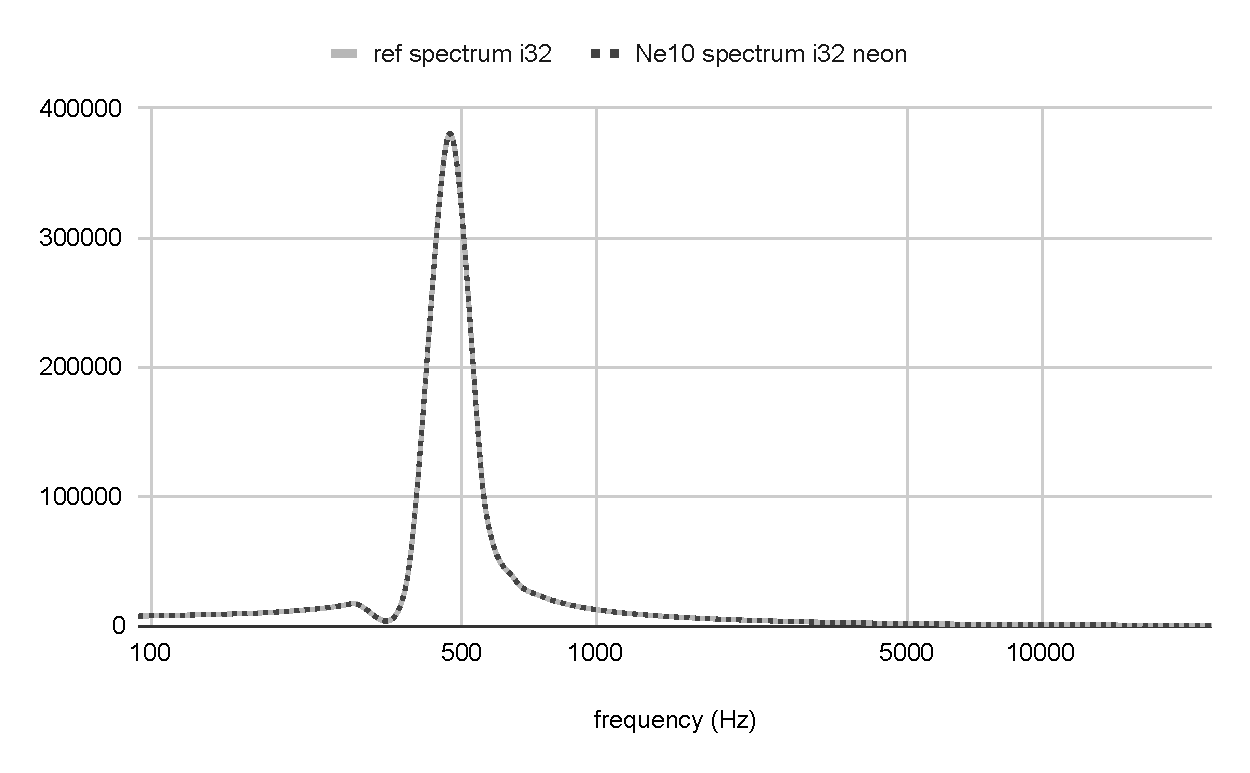
\includegraphics[width=.8\linewidth]{./images/validation_ne10_i32_neon.pdf}
        \caption{Spectre de fréquences généré par la MDCT Ne10 i32 Neon comparé au spectre de référence}
        \label{fig:validation_ne10_i32_neon}
    \end{figure}


    \newpage
    \section{Analyse des résultats}
    \subsection{Validation des données}
    \label{sec:validation}

        % \paragraph{}% TODO
    % Explication de la lecture des résultats, calcul des bandes de fréquences représentées. Mise en évidence qu'on a bien une seule composante fréquentielle comme attendu pour un signal single tone

    % \begin{itemize}
    %     \item sortie des données et générations de graphiques avec gnuplot
    %     \item résolution en fréquence pour une fenetre de 1024 samples pour un signal échantillonné à 48kHz : sur les graphiques $\frac{48000}{1024} = \SI{46.875}{\hertz}$ 1.3333... ms -> f = 1 / 1.33333 = 750 Hz OU res = fs / samples -> sur les graphiques on a des raies de fréquence de 750 Hz. Pour une fenêtre de 1024 = Hz
    % \end{itemize}
    % Graphiques sur sinusoide simple : augmenter la fréquence (i * qch pour déplacer la bande de fréquence), 


    \paragraph{}
    Les sections précédentes ont montré que la les différentes itérations de la MDCT développées ont été validées à chaque étape. Cette validation consiste essentiellement en une vérification manuelle des données de sortie de la MDCT : avec un signal sinusoïdal connu en entrée, il est facile de vérifier que l'analyse fréquentielle ne contient bien qu'une seule composante fréquentielle, que la vérification se fasse en lisant les données brutes à la sortie de l'algorithme ou par une analyse graphique de celle-ci.

    % \paragraph{}
    %La MDCT a également été validée par comparaison de ses données de sortie avec des algorithmes de référence : les implémentations de la formule mathématique de la MDCT présentée dans les annexes \ref{an:ref_mdct_float} pour l'implémentation en arithmétique \emph{floating point} et \ref{an:ref_mdct_int} en \emph{fixed point}.

    \paragraph{}
    Ces tests auraient pu être améliorés en automatisant la vérification, e.g. en générant une fois les données de référence attendues pour permettre le développement d'un code de test qui compare automatiquement les données de références avec les données à vérifier. En effet, devoir relancer les tests et vérifier les données à chaque fois qu'une modification est faite dans le code peut s'avérer laborieux et mettre en place des tests automatiques aurait permis de gagner un temps précieux.


    %     Réaliser une fonction qui calcule la somme des cosinus (formule de wikipedia) pour chaque samples (pas du tout optimisée donc super lente). Pour la calcul en integer, on peut autoriser un manque de précision de max 1 LSB.



    % \paragraph{}
    % Pour les codecs c'est important de garder l'implémentation de référence mais à un moment on ne peut plus tester sur l'architecture intel. En pratique on utilise des pointeurs de fonction à déréférencer pour appeler l'implémentation voulue. En fonction du CPU ID, on sait quelles instructions on utilise. Au runtime, on choisit une ou l'autre implémentation en fonction de l'architecture, e.g. certains ARM n'ont pas les routines NEON

    % one algorithm to compare them all


    % donner un exemple avec plusieurs composantes fréquentielles



    \subsection{Gain en performance}
    \label{sec:mdct_perfs}
    \paragraph{}
    La mesure des performances a pour but de valider le bloc MDCT avant de l'intégrer au codec AAC. Le cahier des charges du stage ne contenait pas d'objectif à atteindre en terme de performances, ni absolu (e.g. un temps d'exécution maximal à respecter dans des conditions données), ni relatif (e.g. gagner un certain pourcentage de performances par rapport à une MDCT de référence).

    \paragraph{}
    L'objectif en terme de temps d'exécution n'étant pas fini, il a été décidé de tenter de gagner le maximum de performances sur le temps de mon stage. Le critère de réussite est dès lors d'obtenir des performances au moins équivalentes pour la version finale de la MDCT que pour ses itérations précédentes.

    \paragraph{}
    Le temps d'exécution de la MDCT \emph{fixed point} doit évidemment être inférieur au temps d'exécution de l'algorithme de référence puisque celui-ci ne contient aucune optimisation. Ce temps peut toutefois être équivalent au temps d'exécution de la MDCT \emph{floating point} : à performances équivalentes, l'algorithme \emph{fixed point} rendra tout de même l'encodeur AAC plus performant en économisant les transtypages \emph{integer}-\emph{floating point} à l'entrée et à la sortie du bloc MDCT. En effet, les données sont reçues par la MDCT en \emph{integer} et devront être traitées en \emph{integer} par le bloc de quantification à la sortie de la MDCT.

    \paragraph{}
    Le temps d'exécution des différentes itérations de la MDCT a été mesuré sur base du code de l'\textbf{annexe TODO} compilé par les commandes CMake présentées dans l'annexe l'\textbf{annexe TODO}. Le code permet de générer plusieurs exécutables en fonction de la variable de préprocesseur définie à la compilation, afin de pouvoir tester :
    \begin{itemize}
        \item La MDCT \emph{Ne10 float 32 plain C};
        \item La MDCT \emph{Ne10 integer 32 plain C};
        \item La MDCT \emph{Ne10 integer 32 neon};
        \item La MDCT de référence en \emph{float 32}.
    \end{itemize}

    \paragraph{}
    Le code de l'\textbf{annexe TODO}, compilé avec les commandes de l'\textbf{annexe TODO} génère un exécutable permettant de mesurer le temps moyen d'exécution de la MDCT \emph{FFTW3 float 32}.
    
    \paragraph{}
    Les tests de performances sont lancés sur le Raspberry via une connexion SSH. Un script permet d'appeler tous les exécutables avec les paramètres voulus et les résultats affichés en console sont rediirigés vers un fichier texte. Les tests sont réalisés en isolation, i.e. aucun processus non nécessaire au fonctionnement du Raspberry n'est lancé durant la réalisation des tests pour ne pas interférer et risquer d'allonger le temps d'exécution. Les mesures de performances ont été prises avec des exécutables compilés en mode \emph{release} avec l'option \texttt{CMAKE\_BUILD\_TYPE=RELEASE}.

    \paragraph{}
    Les résultats présentés dans la table \ref{tab:perf_mdct} ont été mesurés sur \SI{10000000}{} d'exécutions (\SI{10000}{} pour l'algorithme de référence). Afin de ne pas introduire d'alétoire dans ces mesures, les MDCT ont toutes été testées avec le même signal temporel en entrée : un signal sinusoïdal à \SI{440}{\hertz}.

    \begin{table}[H]
        \centering
        \begin{tabular}{ l | D{.}{.}{-1} | D{x}{\times}{-1} }
            \multicolumn{1}{c|}{\textbf{MDCT}} & \multicolumn{1}{M{3cm}|}{\textbf{Temps d'exécution moyen (ns)}} &\multicolumn{1}{c}{\textbf{Écart type (ns)}} \\
            \hline
            \emph{Ne10 i32 Neon}   &  5796.35              & 0.02259 x 10^{-6} \\
            \emph{Ne10 i32 C}      & 22066.8               & 3.31025 x 10^{-6} \\
            \emph{Ne10 f32}        &  9020.1               & 0.02251 x 10^{-6} \\
            \emph{FFTW3 f32}       &  7446.84              & 1.29403 x 10^{-6} \\
            \emph{Reference f32}   & 29212.6 \times 10^3   & 0.77552 x 10^{-6} \\
        \end{tabular}
        \caption{Test de performance des algorithmes MDCT}
        \label{tab:perf_mdct}
    \end{table}
    % TODO ajouter plus de données -> demander si des fréquences sont plus intéressantes que d'autre

    \paragraph{}
    Les résultats montrent que la MDCT optimisée avec les instructions SIMD Neon est bien plus rapide que les autres MDCT développées avec un temps d'exécution moyen de \SI{5796.35}{\nano\second}. L'objectif du stage est donc bien atteint.

    \paragraph{}
    L'algorithme MDCT de référence est le plus lent de tous avec un temps d'exécution moyen de \SI{29212.6}{\micro\second}. Ce résultat est tout à fait normal puisque cet algoritme a été développé sans optimisation particulière.

    \paragraph{}
    La MDCT \emph{fixed point} en \emph{plain C} est la plus lente des MDCT optimisées avec un temps d'exécution moyen de \SI{22066.8}{\nano\second}. La section \ref{sec:fixed_point_perfs} permet de comprendre en quoi ce résultat est cohérent puisque l'architecture ARMv7 supporte de nombreuses instructions en \emph{float} sur 32 bits et que l'arithmétique \emph{fixed point} nécessite souvent plusieurs opérations là où une seule est nécessaire en \emph{floating point}.

    \paragraph{}
    Ces résultats montrent que l'implémentation des fonctions SIMD Neon était nécessaire afin d'obtenir des performances acceptables. Sans l'implémentation d'une MDCT optimisée avec ces instructions, l'utilisation d'une MDCT \emph{fixed point} aurait été compromis par les résultats insatisfaisants de l'implémentation \emph{plain C}.

    \paragraph{}
    Enfin, pour les implémentation \emph{floating point plain C}, la MDCT \emph{Ne10} est un peu plus lente que la MDCT \emph{FFTW3} avec un temps d'exécution moyen de \SI{9020.1}{\nano\second} contre \SI{7446.84}{\nano\second}. Ce résultat est cohérent avec les performances des différentes FFT mesurées à la section \ref{sec:fft_perfs} : la FFT de \emph{FFTW3} en \emph{float 32} est en effet environ \SI{2}{\micro\second} plus rapide que la FFT de \emph{Ne10} en \emph{float 32 plain C}.




 
    % Comparaison avec un implémentation de référence plain c mais aussi à titre indicatif avec l'algorithme de référence car le plain c est déjà optimisé


    % L'impact de la window function : exemple avec un sinus : les composantes fréquentielles du sinus ressortent beaucoup mieux.

    % +difficultés au niveau des performances pas bonnes jusqu'à la fin

    % projet compilé en release pour les tests de perf

    \subsection{Perte de précision}
    % Comparaison avec l'algorithme de référence
    % Annexe : algo de référence, test de comparaison, résultats avec des données aléatoires et avec un sinus simple
    % ce serait mieux de voir la perte de précision sur tout l'encodeur mais c'est déjà une indication, maintenant est-ce que ç aprête tellement à conséquence ?




    \newpage
    \section{Améliorations possibles}
    \label{sec:ameliorations}
    \begin{itemize}
        \item Fonction fenêtre intégrée aux opérations de pre twiddling
        \item Quantification intégrée au post twiddling
        \item tests automatisés
        \item code en C
        \item tests de performances plus poussés avec comparaison avec un algo existant
    \end{itemize}
    % Améliorations encore possible : faire les premières opérations de prétwiddling en Q15 8 par 8 avant de splitter, mêler les facteurs de la fenêtre aux facteurs de twiddling
    % Pas trop de C++ parce que faire un objet avec plein d'accessors, ce n'est pas très optimisé (on se retrouve avec un gros objet avec plein de variables). Derrière on fait de l'assembleur => il y a un trop grand écart. D'habitude les codesc audio sotn codés en C mais c'est aussi peut-être juste pour une raison historique.


    % \paragraph{Points d'attention}
    % \begin{itemize}
    %     \item alignement des tableaux (souvent c'est une contrainte imposée car permet facilement d'optimiser du code) : résolutions possibles en allouant dynamiquement les tableaux et en jouant avec une arithmétique de pointeur OU utilisation de posix mem align...
    % \end{itemize}

    % Attention à la manière d'écrire le code. Ici on n'a pas besoin de faire attention à ce que le compilateur puisse faire du inline (ex remplacer l'appel à z = add(a, d) par z = a+d pour économiser le call) car l'algo est déjà très optimisé -> pas d'optimisations de compilateur possible et en plus on a une grosse routine -> économiser un call n'est pas forcément intéressant.

    \newpage
    \section*{Conclusion}
    \addcontentsline{toc}{section}{\protect\numberline{}Conclusion}
    \paragraph{}
    Sur base du cahier des charges de début de stage, il a été décidé que mon travail s
    % Résultats obtenus + améliorations possibles

    \newpage
    \bibliography{biblio} 
    \bibliographystyle{ieeetr.bst}
    \addcontentsline{toc}{section}{\protect\numberline{}Références}

    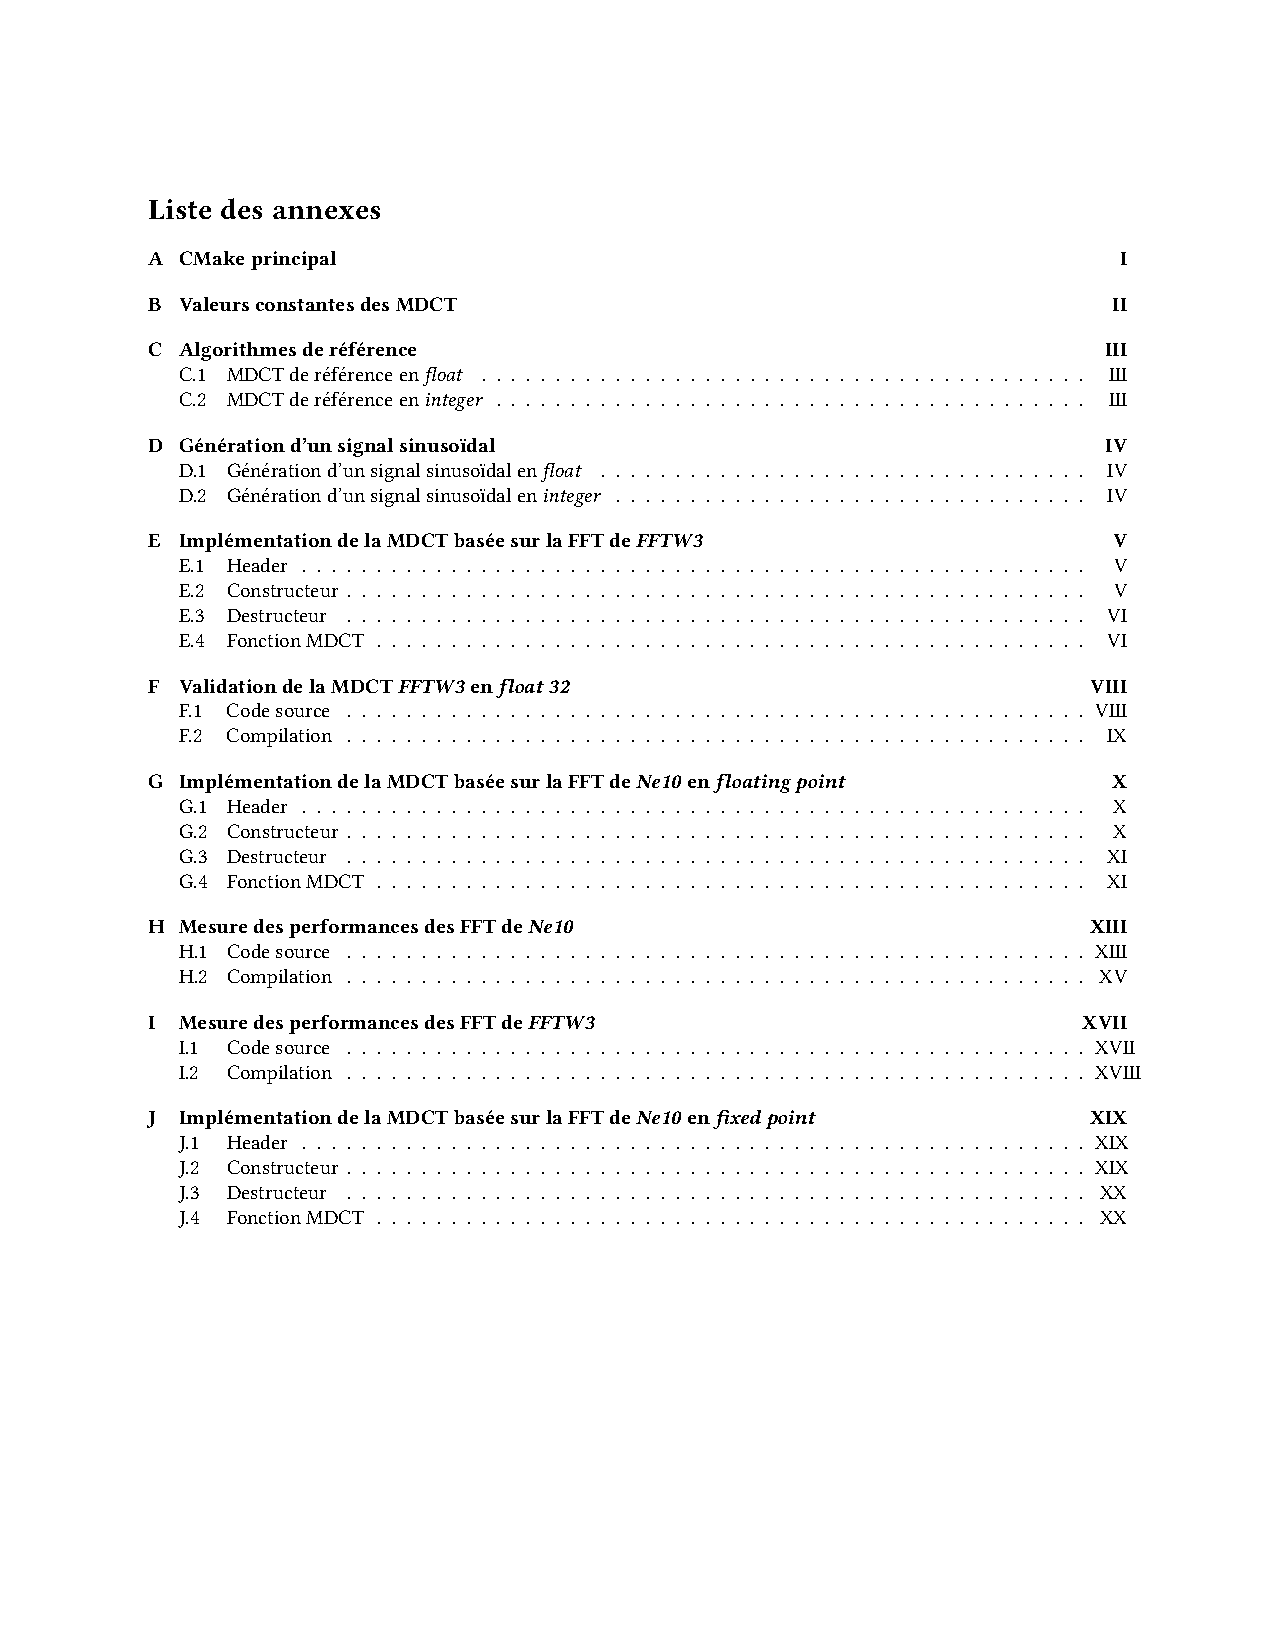
\includepdf[pages=-]{annexes}

\end{document}
